%!TEX root = ../thesis.tex
%*******************************************************************************
%****************************** Second Chapter *********************************
%*******************************************************************************
\chapter{Severity estimation}\label{cha:hospitalseverity}

\graphicspath{{03_HospitalSeverity/Figs/}}

Compared to the infection fatality rate (IFR) and case fatality rate (CFR) introduced in Chapter~\ref{cha:introduction}, the hospitalised fatality risk (HFR)\nomenclature[z]{HFR}{Hospitalised fatality risk} has a better-defined denominator (admission to hospital). In the UK, hospital admissions for COVID-19 were subject to significantly less reporting bias than infections among the general population, due to centralised and high-quality reporting systems. Nonetheless, the case-mix at hospital admission can vary substantially and the presence of competing risks and other biases may lead to distorted estimates unless these factors are addressed.

\section{Aims of this chapter}

A segment of the population who acquire SARS-CoV-2 in the community will require hospitalisation, potential escalation to intensive care facilities, and may die in hospital or soon after discharge. Knowledge of the risks of the different hospital pathways experienced by COVID-19 patients, the lengths of stay in hospital prior to a final outcome, and how these change over time, are crucial to:\ (i) evaluate the effect of clinical and public health strategies on reducing disease burden (e.g.\ by reconstructing the evolution of the pandemic); and (ii) inform future policies, through medium and long-term predictions of hospital demand~\parencite{Birrell2021-pu, Scientific_Pandemic_Influenza_Group_on_Modelling_Operational_sub-group2021-il}.

In this chapter I aim to apply multi-state models to estimate trends in hospital pathways and outcomes among patients hospitalised with community-onset COVID-19 during the initial waves of the pandemic. In the first analysis I investigate the changing risks of different pathways through hospital over the first two waves (i.e.\ first 12-months) of the pandemic in England, prior to widespread vaccination. In the second analysis I estimate the longer-term changes in HFR and hospital lengths of stay including the third wave (i.e.\ first 26-months), according to vaccination status and hospital load. Both analyses account for competing risks and censoring due to missing outcome information.

\section{Background}

\subsection{Timeline of COVID pandemic measures}

In England, the first cases of COVID-19 were detected in March 2020 and the country experienced three distinct `waves' of infection over the following two years (Figure~\ref{fig:pandemic-waves}). By the end of April 2022, there had been over 18 million confirmed cases of COVID-19 in England, resulting in 730,000 hospital admissions, and 190,000 people had died with COVID-19 on their death certificate~\parencite{UK_Government2021-ip}.

\begin{figure}[htbp!]
    \centering
    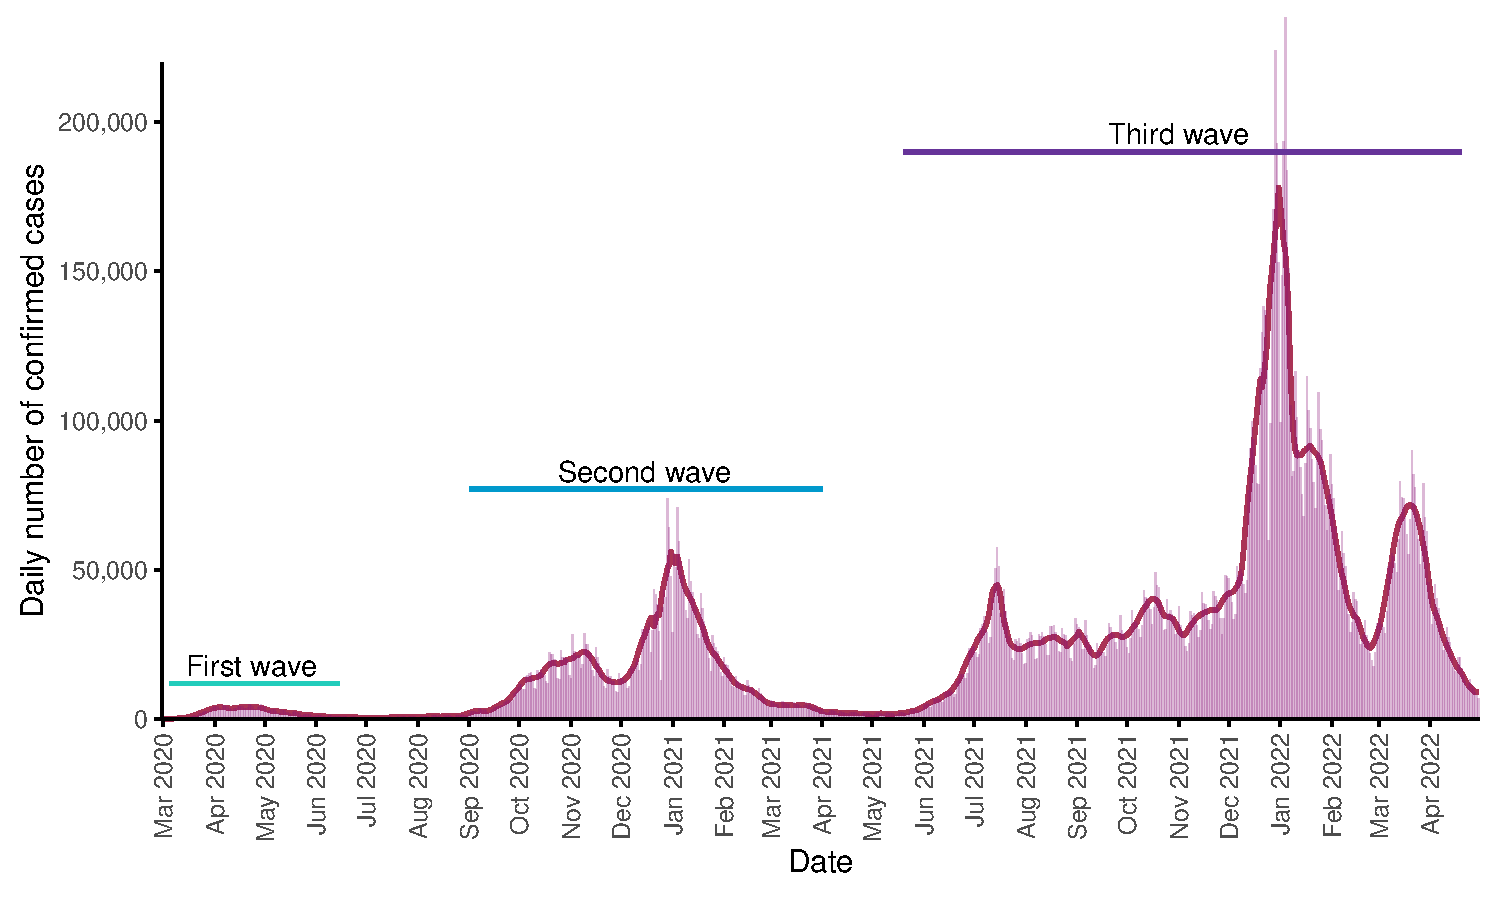
\includegraphics[width=\textwidth]{pandemic_waves.pdf}
    \caption[Daily number and 7-day average of confirmed SARS-CoV-2 cases over successive pandemic waves]{Daily number and 7-day average of confirmed SARS-CoV-2 cases over successive pandemic waves, March 2020 to April 2022, data from the UK Health Security Agency~\parencite{UK_Government2021-ip}.}\label{fig:pandemic-waves}
\end{figure}

The various interventions introduced during the first wave of COVID-19 pandemic, such as testing and social distancing, are described in Section~\ref{sec:prevention-strategies}. Over the same period, hospitals were reconfigured in recognition of the severity of illness among people presenting to emergency care. An example of this was an scale up in the number of intensive care unit (ICU)\nomenclature[z]{ICU}{Intensive care unit} and high dependency unit (HDU)\nomenclature[z]{HDU}{High dependence unit} beds, with more than 3500 mechanical ventilation beds occupied in January 2021~\parencite{UK_Government2021-ip}.

COVID-19 vaccination began in December 2020, initially prioritised to those most at risk of adverse outcomes and later offered to all adults. Widespread vaccination has been highly effective in reducing the risk of hospitalisation, morbidity, and mortality for those who become infected~\parencite{Lopez_Bernal2021-gt,Public_Health_England2021-xs, Nyberg2022-jz}.

\subsection{Measures of severity}

The HFR considers only those who are ill enough to require hospital admission, so is likely to be much higher than either the IFR or CFR\@. Other measures of severity related to the HFR may look at endpoints other than death, e.g.\ the risk of hospital or critical care admission. Severity can also be quantified as a time delay, such as the time from infection to recovery, with a longer delay indicating greater severity. In these analyses, infection time is typically unknown and delays from measurable events, such as the date of symptom onset or date of first positive test, are used~\parencite{Nyberg2021-cr, Harrison2020-iw}. Electronic hospital records (EHR)\nomenclature[z]{EHR}{Electronic hospital record} and hospital surveillance data can similarly be used to estimate delays, for instance the delay from admission to critical care admission, or from admission to final outcome.

Regardless of which metric is used, or which timescale considered, severity measurement is often subject to bias as a result of:\ incomplete case-ascertainment, changes in the frequency of testing and healthcare monitoring, differences in population-level immunity, and variation in case-mix over time~\parencite{Bhattacharya2021-wq}. Studies of HFR are also typically not representative of the general population, since they do not consider the disproportional burden of infection on certain groups. Controlling for and assessing the potential impact of these biases can help to ensure accuracy in severity estimates.

Finally, as the evolution of new variants, immunity acquired through past infection or vaccination, and improved therapeutics may all lead to changes in disease severity over time, regular updates of severity are important for national policy makers, and a crucial input to models reconstructing pandemic evolution and predicting hospital demand~\parencite{Birrell2021-pu, Birrell2021-ou}.

\subsection{Severity estimation}

During the first wave of infections in England, COVID-19 was observed to disproportionately impact older people and those with multiple co-morbidities, compared to younger, healthier individuals~\parencite{Williamson2020-xk, Public_Health_England2020-xu}. Preliminary evidence among those admitted to hospital in England and Scotland demonstrated that these factors, alongside sex, ethnicity, and socioeconomic deprivation, also heavily influenced an individual's prognosis following hospital admission for COVID-19~\parencite{Ferrando-Vivas2021-ut, Docherty2021-es, Agrawal2021-ee, Gray2021-xk, Mathur2021-zf}.

The studies referenced above investigated the effect of different covariates on COVID-19 HFR, with Cox proportional hazards models used to estimate hazard ratios in two studies~\parencite{Ferrando-Vivas2021-ut, Mathur2021-zf}, and logistic regression used to estimate odds ratios in several others~\parencite{Agrawal2021-ee, Gray2021-xk, Docherty2021-es}. Most included age, sex, ethnicity, socioeconomic deprivation, and comorbidity, with a few using cubic splines to model covariates with non-linear effects, particularly age~\parencite{Mathur2021-zf, Gray2021-xk, Ferrando-Vivas2021-ut}.

\subsubsection{Limitations}

Data collection mechanisms were a limitation in many of these studies, with most datasets only receiving information on completed hospital episodes (i.e.\ at death or discharge), and reporting of these completed episodes may also have been subject to delay. This issue is known as right-truncation, and, if not correctly accounted for, may bias HFR and length of stay estimates, as discussed in Section~\ref{sec:censoring-truncation}. \cite{Seaman2022-wg} have presented several methods to account for right-truncation when estimating time-to-event distributions in the context of an infectious disease epidemic.

Most of the studies performed administrative right-censoring of patient follow-up times by only considering cases which had experienced an outcome within 28 (or 30) days of hospital admission~\parencite{Docherty2021-es, Agrawal2021-ee, Ferrando-Vivas2021-ut}. Whilst right-censoring of patient follow-up is common in survival studies, this relatively short censoring window may ignore information on patients with more complex needs, who spend longer in hospital prior to a final outcome, and truncated patient stays would be completely excluded.

These studies also mostly focused on the first wave of the pandemic, and tended not to explicitly include calendar time as a covariate. The Intensive Care National Audit \& Research Centre (ICNARC)\nomenclature[z]{ICNARC}{Intensive Care National Audit \& Research Centre}, which considered a longer period, reported that the mortality risk for patients admitted to intensive care in England had dropped throughout the first wave, but increased into the start of the second wave~\parencite{Intensive-Care-National-Audit-and-Research-Centre2021-vs}. While extending to longer time periods is desirable, the case mix of people presenting to hospital has varied throughout the pandemic and improvements have been made in therapies for COVID-19. Studies which extend to longer time periods should, therefore, consider the impact of collider bias (see Section~\ref{sec:observational-bias}), mentioned as a limitation by~\cite{Gray2021-xk}.

None of these initial studies considered the impact of hospital load on COVID-19 outcomes. A study by the King’s Fund concluded that a shortage of overnight and acute bed availability prior to the pandemic had already put hospitals under increased strain~\parencite{Ewbank2021-hi}. A study across 207 hospitals during the pandemic found that ICU strain was associated with higher acute hospital mortality~\parencite{Wilcox2022-yr}, and similar findings have been reported in Switzerland, where an ICU occupancy of 70\% or greater was estimated to be a tipping point at which outcomes become adversely affected~\parencite{Anderegg2022-tq}.

\section{COVID-19 surveillance data}\label{sec:covid-hosp-data}

Surveillance of the emergence and ongoing variation in the SARS-CoV-2 virus has been vital for public health monitoring during the COVID-19 pandemic. In England during March 2020, hospital surveillance data systems were swiftly reconfigured to collect information specifically related to COVID-19 admissions. Data from two of these systems will be described in further detail in this section.

\subsection{Hospital surveillance data}

Data from two hospital surveillance systems were available:\ a case-reporting dataset from a subset of sentinel clinics with patient details uploaded upon admission and updated in real-time; and a nationally representative dataset of all hospital admissions, with a reporting delay as records were only reported at final hospital outcome (i.e.\ at death or discharge). These datasets collected a wide array of data from the point of hospital admission to enable assessment of infection severity following hospitalisation.

As the focus for these analyses was understanding the severity and impact of community-acquired COVID-19, hospital-onset (or nosocomial) COVID-19 cases were excluded. Those with hospital-onset infection tended to be older and have longer lengths of stay than the community-onset cases, and transmission dynamics were likely to be significantly different for hospital-acquired as compared to community-acquired cases~\parencite{Cooper2023-sp, Evans2022-ob}.

\subsubsection{SARI-Watch}

The Severe Acute Respiratory Infections in England (SARI-Watch), previously known as the COVID-19 Hospitalisations in England Surveillance System (CHESS), is run by UKHSA and collects detailed individual-level data on hospital admissions for COVID-19 and influenza from a subset of sentinel NHS trusts in England, with mandatory reporting of admissions to ICU (and HDU)~\parencite{Public_Health_England2021-ao}.

Data are reported in real-time via a secure online reporting tool, with data reporters able to update records as changes in care pathways and/or hospital outcomes occur. Covariate information collected in SARI-Watch includes dates of hospital and critical care admission, date and type of outcome, baseline characteristics, and NHS number.

As above, data were limited to admissions for non-nosocomial (i.e.\ community-acquired) admissions to sentinel NHS trusts with known admission and discharge or death date, or right-censored at the date of extraction.

\subsubsection{SUS}

The NHS England Secondary Uses Service (SUS) dataset, run by NHS England, contains well-completed, individual-level data on hospital admissions for COVID-19 across all NHS trusts in England. SUS data are only reported upon completion of a hospital stay (i.e.\ at the point of discharge from hospital or death) and are therefore subject to a reporting delay. To partially account for this, linkage to the Emergency Care Dataset for England (ECDS), which promptly records all emergency care attendances and onwards destinations (i.e.\ to home or admittance to hospital), may be used to obtain information for patients admitted via emergency care and remaining in hospital~\parencite{NHS-Digital2023-iv}.

Covariate information collected in SUS includes:\ date of hospital admission, age group, Charleson comorbidity index (CCI)~\parencite{Charlson1987-nz}, baseline characteristics, and NHS number. As data on all hospital admissions are collected, a crude measure of demand (or hospital load) can be obtained from these data, e.g.\ the number of admissions within a 1-day period.

\subsection{Data linkage}

Obtaining complete information on a patient's testing history, vaccination status, pathways through hospital, and eventual outcome requires data linkage to augment the hospital records. Both SARI-Watch and SUS collected NHS number, which was the basis for this linkage~\parencite{Bhattacharya2021-wq}. Data validation on the linked datasets was used to rule-out spurious matches, helped to minimise missing data, and improved data quality.

The data available for linkage included:
%
\begin{itemize}
    \item COVID-19 testing data from the UKHSA Second Generation Surveillance System (SGSS)~\parencite{NHS-Digital2024-pu} collected via two routes: \textbf{Pillar 1}, tested on arrival at hospital, and \textbf{Pillar 2}, tested within the community;
    \item vaccination data from the National Immunisation and Vaccine System (NIVS)~\parencite{NHS-Digital2022-vd};
    \item data on deaths from UKHSA's COVID-19 mortality dataset~\parencite{Covid-19_EpiCell2020-uv}. These data comprised deaths from four sources, with death outcomes included if they occurred within 60 days of a positive COVID-19 test, or if COVID-19 was mentioned on the death certificate:
          %
          \begin{enumerate}
              \item Office for National Statistics (ONS) death registrations;
              \item NHS England deaths in hospitals;
              \item SGSS;
              \item local Health Protection Teams.
          \end{enumerate}
\end{itemize}

A third hospital dataset, the NHS Hospital Episodes Statistics (HES), also recorded information on hospital admissions for COVID-19, but due to substantial reporting delay (of >3 months) these data had limited utility for pandemic response~\parencite{NHS_Digital2020-jn}. As HES contains more granular information these data were used for validation, and to minimise missing information.

\section{Pre-vaccine hospitalised severity}

In this section I investigate COVID-19 hospitalised severity during the first two waves (12-months) of the COVID-19 pandemic, pre-vaccine introduction. The aim of this analysis was to assess how competing pathways through hospital, and the corresponding lengths of stay in hospital have changed over time. Changes in the hospital-fatality risk (HFR) and time to final event were estimated using Aalen-Johansen and parametric multi-state mixture models.

\subsection{Data}

The SARI-Watch data include all dates of movement between levels of care (e.g.\ Hospital/ICU), a patient's current status (e.g.\ still in hospital/still in ICU/transferred/unknown) or final outcome (e.g.\ discharged/died/unknown), and detailed information on patient characteristics. Data for March 2020 to February 2021 were extracted at the end of March 2021, with data linkage to the UKHSA mortality dataset and HES used to improve the completeness of outcome information and patient characteristics.

Figure~\ref{fig:sari-icu-admission} panel A shows the final outcomes and information on missing outcomes for patients reported in SARI-Watch between March 2020 and February 2021, and panel B shows the proportion of patients who were admitted to ICU over this period.

\begin{figure}[htbp!]
    \centering
    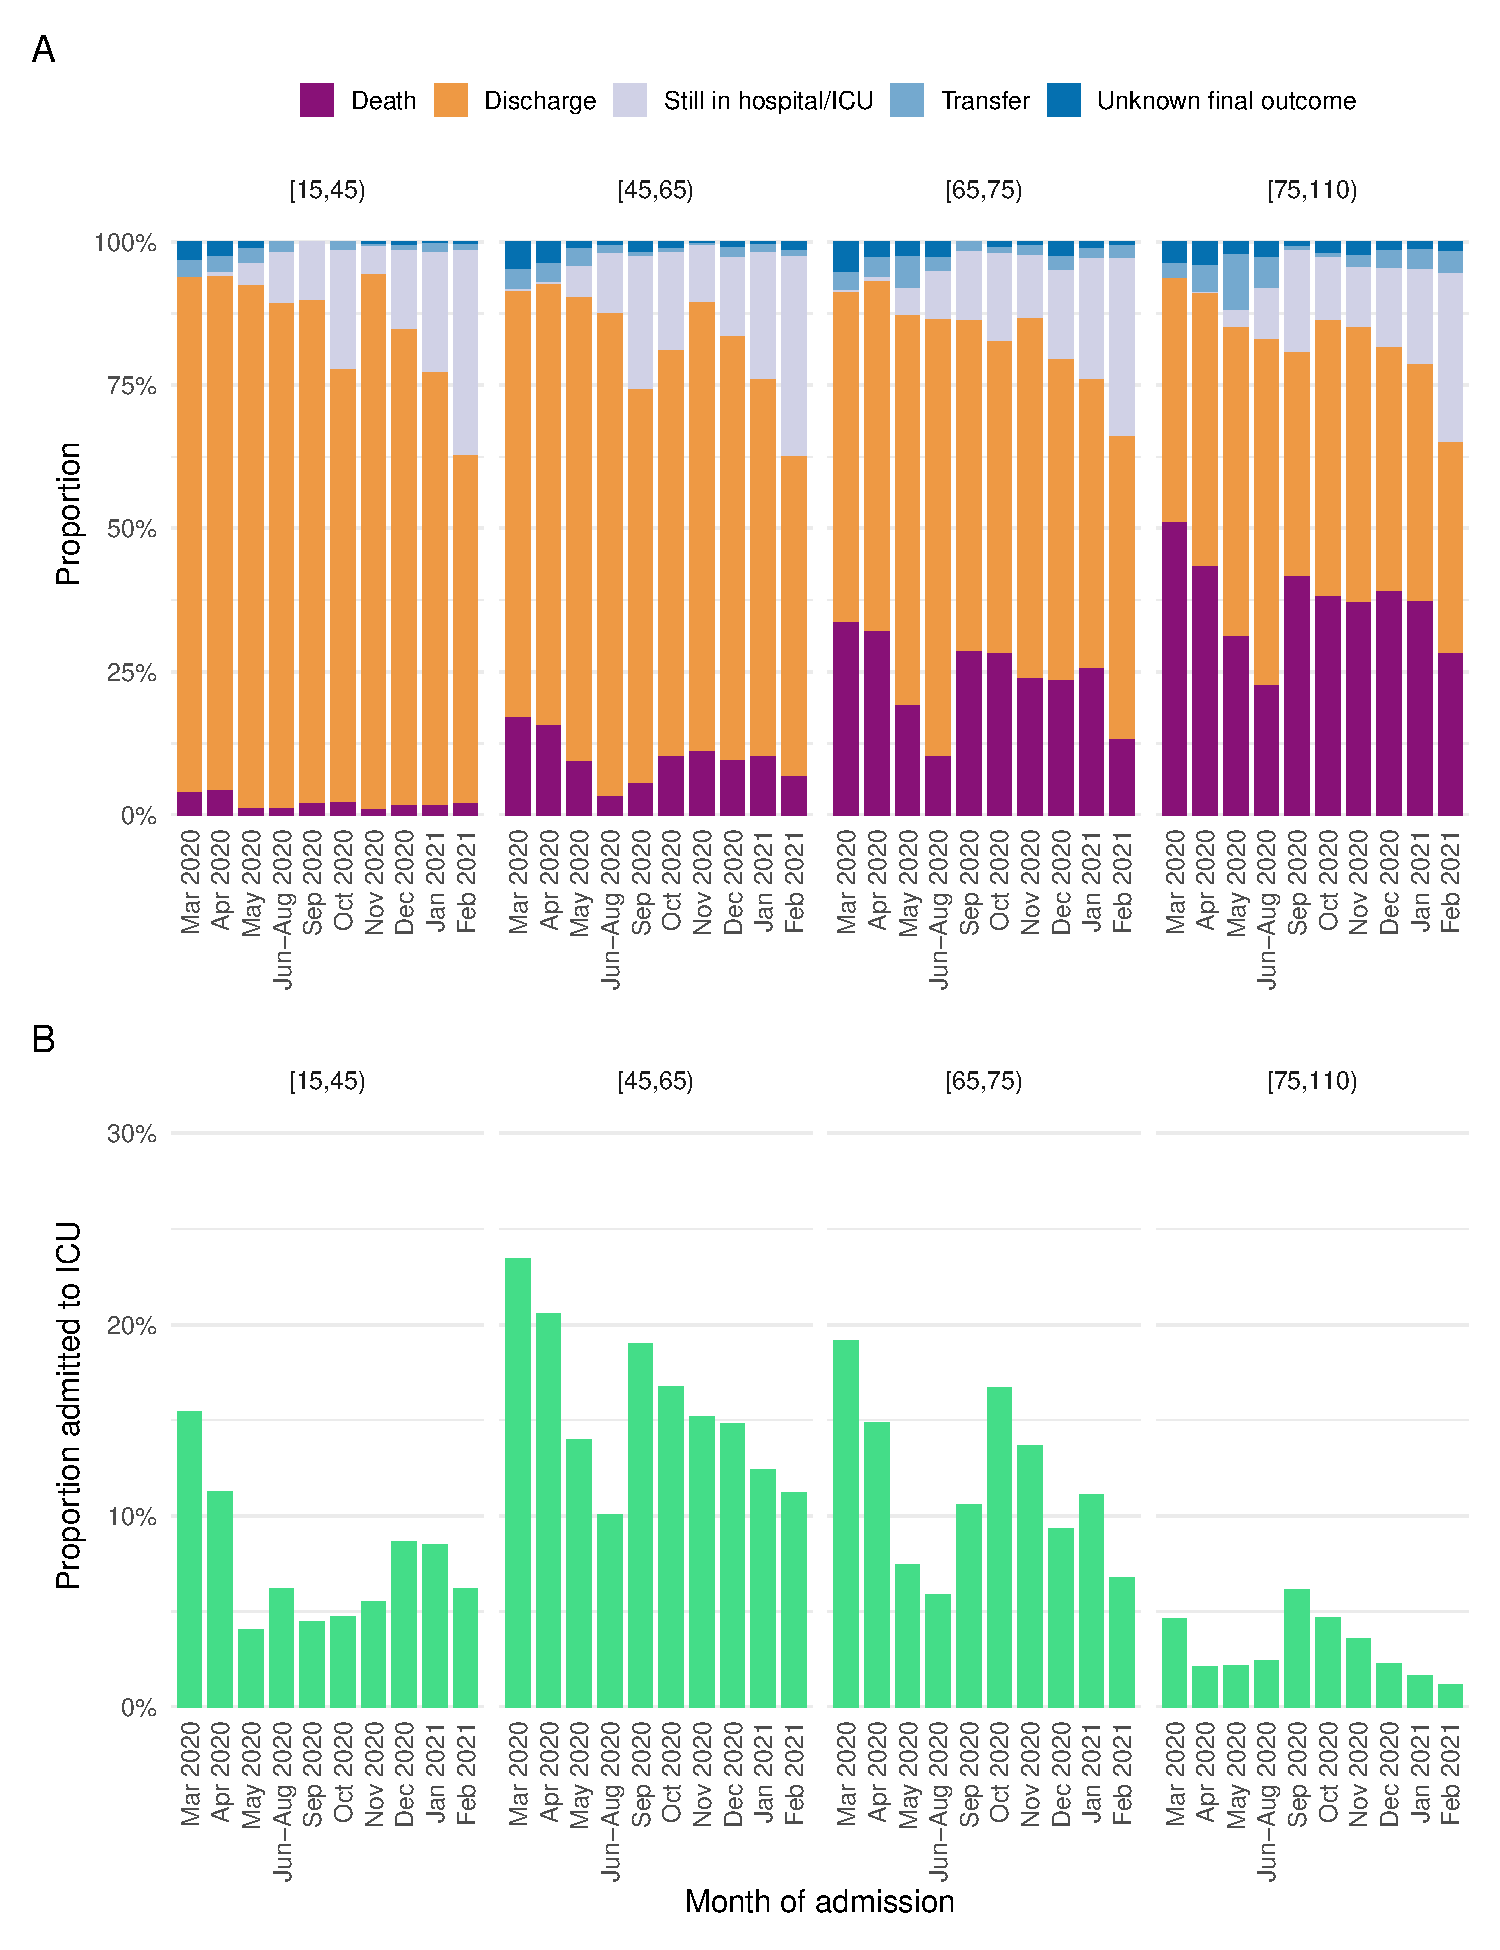
\includegraphics[width=\textwidth]{sari_icu_admission.pdf}
    \caption[Proportion of COVID-19 hospital admissions by age group, final outcome, and ICU admission status]{Proportion of COVID-19 hospital admissions by age group and final outcome (Panel A), and ICU admission status (panel B), March 2020 to February 2021. Admissions occurring during June, July and August 2020 are grouped due to small numbers.}\label{fig:sari-icu-admission}
\end{figure}

\subsubsection{Censoring}

For this investigation data were updated in real-time and outcomes may have been unknown either (a) because the outcome was not reported despite having occurred (termed `truly missing'), or (b) because the outcome had not occurred by the end of the period covered by the data (`right-censoring'). For past admissions (several months prior), unknown outcomes are more likely to be truly missing, as the majority of patients will have completed their hospital episode. In more recent months, unknown outcomes are more likely to represent patients who remain in hospital care, i.e.\ right-censoring.

The last known status for each patient was used to determine an appropriate cut-off for censoring. Patients reported as `still in hospital/still in ICU' were right-censored at the date of data extraction, or at 60 days if they were reported as still in non-critical care beyond 60 days, or at 90 days if they were reported as still in critical care beyond 90 days. This approach was a compromise between excluding these records from the analysis, which may bias outcome estimation, and censoring at the date of data extraction, which would allow for unrealistically long hospital stays of several months after admission. Transferred patients with unknown outcomes were censored at the date of transfer, patients with unknown status and unknown outcome were censored at the date of their last observed event.

Figure~\ref{fig:sariwatchtransitions} shows the different transitions experienced by individuals in the SARI-Watch data, with right-censoring and missing outcomes indicated.

\begin{figure}[htbp!]
    \centering
    \footnotesize
    \begin{tikzpicture}
        % Nodes
        \node[state, align=center] (hosp) at (0,0) {Hospital\\20,785};
        \node[state, align=center] (icu) [right = 20mm of hosp] {ICU\\2213};
        \node[state, align=center] (dis) [above right = 14mm and 25mm of icu] {Discharged\\12,355};
        \node[state, align=center] (die) [below right = 14mm and 27mm of icu] {Died\\5195};
        \node[state, align=center] (h2) [above = 8mm of dis] {Still in hospital\\1867};
        \node[state, align=center] (i2) [right = 25mm of icu] {Still in ICU\\216};
        \node[state, align=center] (eof) [right = 35mm of i2] {End of follow-up\\19,469};

        % Edges
        \path (hosp) edge[bend left = 30] node[fill=white, align = center] {1867\\(9.0\%)} (h2);
        \path (hosp) edge[bend left = 20] node[anchor=center, fill=white, align = center] {11,435\\(55.0\%)} (dis);
        \path (hosp) edge node[anchor=center, fill=white, align = center] {2213\\(10.6\%)} (icu);
        \path (hosp) edge[bend right = 20] node[anchor=center, fill=white, align = center] {4294\\(20.7\%)} (die);
        \path (hosp) edge[bend right = 57] node[anchor=center, fill=white, align = center] {Transfer\\510 (2.5\%)} (eof);
        \path (hosp) edge[bend right = 92] node[below, align = center] {Unknown outcome\\466 (2.2\%)} (eof);

        \path (icu) edge[bend left = 20] node[anchor=center, fill=white, align = center] {920\\(41.6\%)} (dis);
        \path (icu) edge[bend left = 20] node[anchor=center, fill=white, align = center] {Transfer\\120 (5.4\%)} (eof);
        \path (icu) edge node[anchor=center, fill=white, align = center] {216\\(9.8\%)} (i2);
        \path (icu) edge[bend right = 20] node[anchor=center, fill=white, align = center] {901\\(40.7\%)} (die);
        \path (icu) edge[bend right = 20] node[anchor=center, fill=white, align = center] {Unknown outcome\\56 (2.5\%)} (eof);

        \path (h2) edge[bend left = 20, dashed] node[fill=white, align = center] {Right-censored\\734 (39.3\%)} (eof);
        \path (dis) edge[bend left = 15] node[anchor=center, fill=white, align = center] {12,355\\(100\%)} (eof);
        \path (i2) edge[dashed] node[anchor=center, fill=white, align = center] {Right-censored\\33 (15.3\%)} (eof);
        \path (die) edge[bend right = 15] node[anchor=center, fill=white, align = center] {5195\\(100\%)} (eof);

    \end{tikzpicture}
    \caption[Flow diagram showing transitions between hospital states and outcomes in the SARI-Watch data]{Flow diagram showing transitions between hospital states and outcomes in the SARI-Watch data, with observed number and proportion of individuals in and moving between each state. Dashed lines indicate right-censoring for individuals reported as `still in hospital' after 60 days or `still in ICU' after 90 days.}\label{fig:sariwatchtransitions}
\end{figure}

\subsection{Multi-state model}

\subsubsection{Model description}

Non-parametric Aalen-Johansen and parametric multi-state mixture models, specified to account for the competing risks of each pathway and missing outcome information were applied to the SARI-Watch data. The multi-state models had four states, with the transition intensities to subsequent states depending on how long a person had spent in the current state, but not on any events before entering the current state (i.e.\ a Semi-Markov model). Two sub-models represented competing risks of the next event (i) from Hospital admission, and (ii) from ICU admission, as shown in Figure~\ref{fig:sariwatchdag}.

\begin{figure}[htbp!]
    \centering
    \begin{tikzpicture}
        % Nodes
        \node[state, align=center] (hosp) at (0,0) {Hospital};
        \node[state, align=center] (icu) [right = 20mm of hosp] {ICU};
        \node[state, align=center] (dis) [above right = of icu] {Discharged};
        \node[state, align=center] (die) [below right = of icu] {Died};

        % Submodel
        \node[] (s) [below right = 3mm and 20mm of dis] {\textbf{Submodels}};
        \node[] (s1a) [below left = 3mm and 9mm of s] {};
        \node[] (s2a) [below = 3mm of s1a] {};
        \node[] (s1) [right = 10mm of s1a] {(i) from Hospital};
        \node[] (s2) [right = 10mm of s2a] {(ii) from ICU};

        % Edges
        \path (hosp) edge (icu);
        \path (hosp) edge (dis);
        \path (hosp) edge (die);

        \path (icu) edge[dashed] (dis);
        \path (icu) edge[dashed] (die);

        \path (s1a) edge (s1);
        \path (s2a) edge[dashed] (s2);

    \end{tikzpicture}
    \caption[Multi-state model for pathways through hospital following admission for COVID-19 in the SARI-Watch data]{Multi-state model for pathways through hospital following admission for COVID-19 in the SARI-Watch data. Arrows indicate transitions between states in each of the submodels:\ (i) from Hospital, and (ii) from ICU.}\label{fig:sariwatchdag}
\end{figure}

\subsubsection{Likelihood for multi-state mixture model}

The likelihood for a competing risks model may be extended to our multi-state model~\parencite{Jackson2022-lt}. For each patient $i$, with event observations indexed by $j$, the transitions between states $r_{i,j}$ and $s_{i,j}$ occurring at time $y_{i,j}$ are observed in the data as one of three types, indexed by $\delta_{i,j}$:
%
\begin{enumerate}
    \item exact transition times:\ $\bm{y}_{i,j} = \{y_{i,j},r_{i,j},s_{i,j},\delta_{i,j}=1\}$, where the transition from state $r_{i,j}$ to state $s_{i,j}$ occurs at time $y_{i,j}$;
    \item right-censoring:\ $\bm{y}_{i,j} = \{y_{i,j},r_{i,j},\delta_{i,j}=2\}$, where follow-up ends while the individual is in state $r_{i,j}$ at time $y_{i,j}$, and the next state and time of transition are unknown;
    \item partially-known outcome:\ $\bm{y}_{i,j} = \{y_{i,j},\delta_{i,j}=3\}$, where it is known whether or not an individual went to ICU, but unknown if they are still in hospital at time $y_{i,j}$.
\end{enumerate}

As in Section~\ref{sec:cr-models}, let $\pi_{r,s}$ be the probability that the next state for an individual $i$ in state $r$ is state $s$ and let $f_{r,s}(. \mid \theta_{r,s})$ be the densities of the parametric distributions for the time to transition from state $r$ to state $s$, given that this transition occurs. The likelihood contributions for each $\delta_{i,j}$ are:
%
\[
    \begin{array}{rl}
        \delta_{i,j}=1 :                         & l_{i,j}=\pi_{r_{i,j}s_{i,j}}f_{r_{i,j}s_{i,j}}(y_{i,j} \mid \theta_{r_{i,j}s_{i,j}})               \\
        \delta_{i,j}=2 :                         & l_{i,j}=\sum_{s\in S_{r}}\pi_{r_{i,j}s}\left(1-F_{r_{i,j}s}(y_{i,j} \mid \theta_{r_{i,j}s})\right) \\
        \delta_{i,j}=3, s \neq \text{Discharge}: & \text{as for } \delta_{i,j}=2                                                                      \\
        \delta_{i,j}=3, s = \text{Discharge}:    & l_{i,j}=\pi_{r_{i,j}s}
    \end{array}
\]

The full likelihood is the product of these likelihood contributions:
%
\[
    L(\bm{\pi}, \bm{\theta} \mid \bm{y}) = \prod_{i,j}l_{i,j}
\]

where $\bm{\pi}$ includes all of the competing event probabilities $\pi_{r,s}$, and $\bm{\theta}$ includes the parameters of the time to transition distributions.

\subsubsection{Parametric distributions}

Figure~\ref{fig:time-distribution} shows the empirical distribution of time to transition (measured in days) from hospital admission to the competing outcomes of ICU admission, death, and discharge.

\begin{figure}[htbp!]
    \centering
    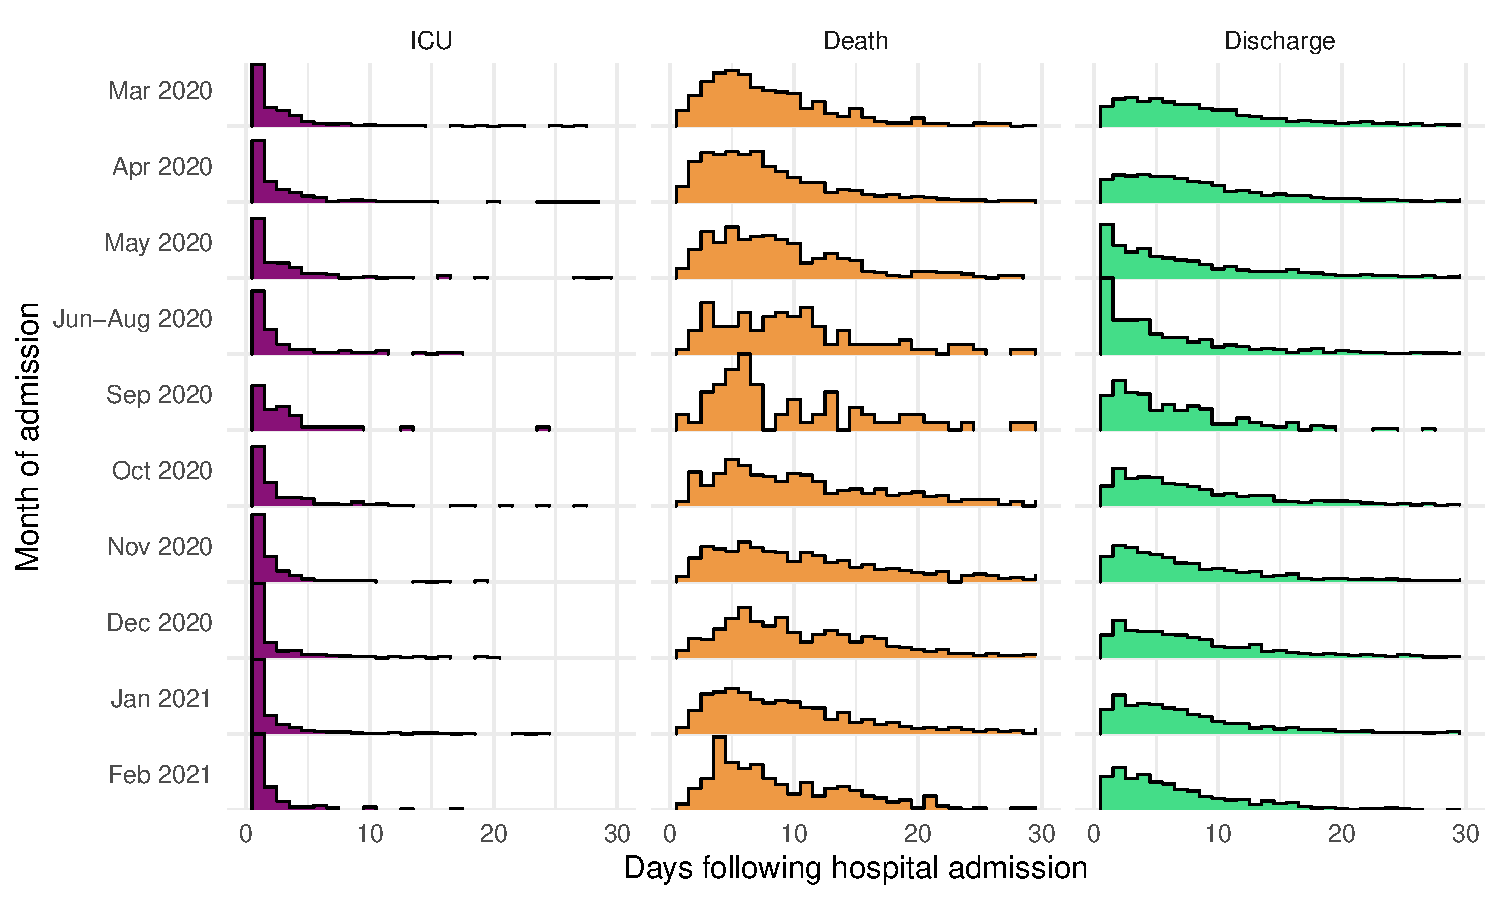
\includegraphics[width=\textwidth]{sari_time_distribution.pdf}
    \caption[Distribution of time to event in SARI-Watch data for the first 30 days following hospital admission, March 2020 to February 2021]{Distribution of time to event in SARI-Watch data for the first 30 days following hospital admission, by month of hospital admission, March 2020 to February 2021. Admissions occurring during June, July and August are grouped due to small numbers.}\label{fig:time-distribution}
\end{figure}

In selecting parametric distributions to model these times to transition a trade-off must be made between over-parameterisation and goodness of fit. The flexibility of an extra parameter can allow for a better fit to the data, but using too many parameters compared to the data may result in parameters being unidentifiable.

Generalized gamma distributions are common choices for right-censored survival data due to their flexibility, which avoids too many assumptions on the shape of the distribution~\parencite{Pal2020-ns}. One parameterisation of this distribution is expressed in terms of the parameters $\mu$, $\sigma$, and $Q$, representing the mean (location), scale, and shape of the distribution, respectively~\parencite{Prentice1974-ec}:
%
\begin{align*}
    f(x \mid \mu, \sigma, Q) = |Q| \frac{{(Q^{-2})}^{Q^{-2}}}{\sigma \cdot x \cdot \Gamma(Q^{-2})} \exp(Q^{-2}(Q\cdot w - \exp(Q\cdot w))) \\
    \text{where } w = \frac{\log(Q^2\cdot g)}{Q}\enspace\text{and}\enspace g \sim \text{Gamma}(Q^{-2}, 1)
\end{align*}

As their name might suggest, generalized gamma distributions are a \textit{generalisation} of other common survival distributions, namely the gamma, log-normal, exponential, and Weibull distributions. These distributions are obtained from the generalized gamma under the following constraints:
%
\[
    \begin{array}{rl}
        \text{Weibull} :     & Q = 1          \\
        \text{Log-normal} :  & Q = 0          \\
        \text{Gamma} :       & Q = \sigma     \\
        \text{Exponential} : & Q = \sigma = 1 \\
    \end{array}
\]

The specification of the mixture model allows for different distributions to be used for each transition. Table~\ref{tab:gof_dist} shows a selection of distributions which were considered for each transition in each of the sub-models, fitted without covariate effects. Goodness of fit and parsimony of each sub-model can be assessed through comparison to non-parametric Aalen-Johansen cumulative incidence curves, likelihood ratio tests, and Akaike information criterion (AIC) values. % why AIC and not BIC? - See Chris' response to reviewers

\begin{table}[!h]
\centering
\caption{\label{tab:gof_dist}Log-likelihood and AIC values for parametric time to transition distributions, sorted by sub-model and AIC. Models with unidentifiable parameters not shown.}
\centering
\begin{tabular}[t]{llllrr}
\toprule
Sub-model & ICU & Death & Discharge & Log-likelihood & AIC\\
\midrule
\cellcolor{gray!10}{Hospital} & \cellcolor{gray!10}{log-normal} & \cellcolor{gray!10}{gengamma} & \cellcolor{gray!10}{gengamma} & \cellcolor{gray!10}{-77841.96} & \cellcolor{gray!10}{155731.93}\\
Hospital & log-normal & log-normal & gengamma & -77843.40 & 155732.80\\
\cellcolor{gray!10}{Hospital} & \cellcolor{gray!10}{log-normal} & \cellcolor{gray!10}{gengamma} & \cellcolor{gray!10}{log-normal} & \cellcolor{gray!10}{-77982.90} & \cellcolor{gray!10}{156011.80}\\
Hospital & Weibull & gengamma & gengamma & -78281.82 & 156611.63\\
\cellcolor{gray!10}{Hospital} & \cellcolor{gray!10}{log-normal} & \cellcolor{gray!10}{gamma} & \cellcolor{gray!10}{gengamma} & \cellcolor{gray!10}{-78324.22} & \cellcolor{gray!10}{156694.44}\\
Hospital & log-normal & Weibull & gengamma & -78329.02 & 156704.05\\
\cellcolor{gray!10}{Hospital} & \cellcolor{gray!10}{log-normal} & \cellcolor{gray!10}{exponential} & \cellcolor{gray!10}{gengamma} & \cellcolor{gray!10}{-78340.72} & \cellcolor{gray!10}{156725.44}\\
Hospital & gamma & gengamma & gengamma & -78367.64 & 156783.28\\
\cellcolor{gray!10}{Hospital} & \cellcolor{gray!10}{exponential} & \cellcolor{gray!10}{gengamma} & \cellcolor{gray!10}{gengamma} & \cellcolor{gray!10}{-78397.36} & \cellcolor{gray!10}{156840.73}\\
Hospital & log-normal & gengamma & Weibull & -79322.13 & 158690.27\\
\cellcolor{gray!10}{Hospital} & \cellcolor{gray!10}{log-normal} & \cellcolor{gray!10}{gengamma} & \cellcolor{gray!10}{gamma} & \cellcolor{gray!10}{-79905.44} & \cellcolor{gray!10}{159856.87}\\
Hospital & log-normal & gengamma & exponential & -81066.20 & 162176.41\\
\cellcolor{gray!10}{ICU} & \cellcolor{gray!10}{} & \cellcolor{gray!10}{gengamma} & \cellcolor{gray!10}{log-normal} & \cellcolor{gray!10}{-8710.57} & \cellcolor{gray!10}{17447.14}\\
ICU &  & gengamma & gengamma & -8710.62 & 17449.24\\
\cellcolor{gray!10}{ICU} & \cellcolor{gray!10}{} & \cellcolor{gray!10}{log-normal} & \cellcolor{gray!10}{gengamma} & \cellcolor{gray!10}{-8717.79} & \cellcolor{gray!10}{17461.59}\\
ICU &  & gamma & gengamma & -8764.12 & 17554.24\\
\cellcolor{gray!10}{ICU} & \cellcolor{gray!10}{} & \cellcolor{gray!10}{gengamma} & \cellcolor{gray!10}{gamma} & \cellcolor{gray!10}{-8765.89} & \cellcolor{gray!10}{17557.78}\\
ICU &  & gengamma & exponential & -8770.58 & 17565.17\\
\cellcolor{gray!10}{ICU} & \cellcolor{gray!10}{} & \cellcolor{gray!10}{gengamma} & \cellcolor{gray!10}{Weibull} & \cellcolor{gray!10}{-8769.90} & \cellcolor{gray!10}{17565.80}\\
ICU &  & exponential & gengamma & -8772.38 & 17568.76\\
\cellcolor{gray!10}{ICU} & \cellcolor{gray!10}{} & \cellcolor{gray!10}{Weibull} & \cellcolor{gray!10}{gengamma} & \cellcolor{gray!10}{-8772.14} & \cellcolor{gray!10}{17570.28}\\
\bottomrule
\end{tabular}
\end{table}


The hospital sub-model with the lowest AIC used a log-normal distribution for the `to ICU' transition and generalized gamma distributions for the `to death', and `to discharge' transitions. The difference in AIC between the two best fitting ICU sub-models was not significant (with a difference in AIC <5), so the generalized gamma distribution was chosen for both transitions based on a comparison to the Aalen-Johansen estimates.

\subsubsection{Covariate effects}

Covariates available in the SARI-Watch dataset included month of admission, age group, sex, region of residence (London, South of England, Midlands and East of England, and North of England), ethnicity, and number of comorbidities (see Table~\ref{tab:sari_characteristics}).

Probabilities of competing events $\pi_{r,s}$ could be related to one or more of these covariates via multinomical logistic regression, with parameters of the time to transition distributions related to covariates through accelerated failure time models, as described in Section~\ref{sec:cr-models}.

For the generalized gamma distribution, covariates can be specified on the mean, scale, and shape parameters, $\mu$, $\sigma$, and $Q$, respectively. For the log-normal distribution, covariates can be specified on the log(mean) and log(standard deviation) parameters, $\mu$ and $\sigma$, respectively. Table~\ref{tab:gof_place} shows the effect on the log-likelihood and AIC of regressing the probability ($\pi$) and the parameters of each time to transition distribution on the month of admission covariate. For example:\ the best-fitting `from Hospital' sub-model included regression on month of admission for each of:
%
\begin{itemize}
    \item the competing event probability ($\pi$);
    \item the mean and scale parameters of the generalized gamma ($\mu$ and $\sigma$);
    \item the log(mean) parameter of the log-normal ($\mu$).
\end{itemize}

\begin{table}[!h]
\centering
\caption{\label{tab:gof_place}Log-likelihood and AIC values for log-normal and generalized gamma distributions, by location of covariate effects, sorted by sub-model and AIC. Models with unidentifiable parameters not shown.}
\centering
\begin{tabular}[t]{lllllrr}
\toprule
Sub-model & $\pi$ & ICU & Death & Discharge & Log-likelihood & AIC\\
\midrule
\cellcolor{gray!10}{Hospital} & \cellcolor{gray!10}{$\checkmark$} & \cellcolor{gray!10}{$\mu$} & \cellcolor{gray!10}{$\mu$, $\sigma$} & \cellcolor{gray!10}{$\mu$, $\sigma$} & \cellcolor{gray!10}{-77328.69} & \cellcolor{gray!10}{154775.39}\\
Hospital & $\checkmark$ & $\sigma$ & $\mu$, $\sigma$ & $\mu$, $\sigma$ & -77330.15 & 154778.30\\
\cellcolor{gray!10}{Hospital} & \cellcolor{gray!10}{$\checkmark$} & \cellcolor{gray!10}{$\mu$} & \cellcolor{gray!10}{$\mu$} & \cellcolor{gray!10}{$\mu$, $\sigma$} & \cellcolor{gray!10}{-77349.89} & \cellcolor{gray!10}{154803.78}\\
Hospital & $\checkmark$ & $\sigma$ & $\mu$ & $\mu$, $\sigma$ & -77351.18 & 154806.35\\
\cellcolor{gray!10}{Hospital} & \cellcolor{gray!10}{$\checkmark$} & \cellcolor{gray!10}{$\mu$} & \cellcolor{gray!10}{$\sigma$} & \cellcolor{gray!10}{$\mu$, $\sigma$} & \cellcolor{gray!10}{-77412.52} & \cellcolor{gray!10}{154929.04}\\
Hospital & $\checkmark$ & $\sigma$ & $\sigma$ & $\mu$, $\sigma$ & -77414.11 & 154932.22\\
\cellcolor{gray!10}{Hospital} & \cellcolor{gray!10}{$\checkmark$} & \cellcolor{gray!10}{$\mu$} & \cellcolor{gray!10}{$\mu$, $\sigma$} & \cellcolor{gray!10}{$\sigma$} & \cellcolor{gray!10}{-77450.65} & \cellcolor{gray!10}{155005.30}\\
Hospital & $\checkmark$ & $\sigma$ & $\mu$, $\sigma$ & $\sigma$ & -77452.02 & 155008.04\\
\cellcolor{gray!10}{Hospital} & \cellcolor{gray!10}{$\checkmark$} & \cellcolor{gray!10}{$\mu$} & \cellcolor{gray!10}{$\mu$} & \cellcolor{gray!10}{$\sigma$} & \cellcolor{gray!10}{-77470.37} & \cellcolor{gray!10}{155030.74}\\
Hospital & $\checkmark$ & $\sigma$ & $\mu$ & $\sigma$ & -77471.77 & 155033.54\\
\cellcolor{gray!10}{Hospital} & \cellcolor{gray!10}{$\checkmark$} & \cellcolor{gray!10}{$\mu$} & \cellcolor{gray!10}{$\sigma$} & \cellcolor{gray!10}{$\sigma$} & \cellcolor{gray!10}{-77534.72} & \cellcolor{gray!10}{155159.44}\\
Hospital & $\checkmark$ & $\sigma$ & $\sigma$ & $\sigma$ & -77535.97 & 155161.95\\
\cellcolor{gray!10}{Hospital} & \cellcolor{gray!10}{$\checkmark$} & \cellcolor{gray!10}{} & \cellcolor{gray!10}{} & \cellcolor{gray!10}{$\sigma$} & \cellcolor{gray!10}{-77561.32} & \cellcolor{gray!10}{155184.63}\\
Hospital & $\checkmark$ & $\mu$ & $\mu$, $\sigma$ & $\mu$ & -77595.90 & 155295.79\\
\cellcolor{gray!10}{Hospital} & \cellcolor{gray!10}{$\checkmark$} & \cellcolor{gray!10}{$\sigma$} & \cellcolor{gray!10}{$\mu$, $\sigma$} & \cellcolor{gray!10}{$\mu$} & \cellcolor{gray!10}{-77596.80} & \cellcolor{gray!10}{155297.60}\\
Hospital & $\checkmark$ & $\mu$ & $\mu$ & $\mu$ & -77615.72 & 155321.45\\
\cellcolor{gray!10}{Hospital} & \cellcolor{gray!10}{$\checkmark$} & \cellcolor{gray!10}{$\sigma$} & \cellcolor{gray!10}{$\mu$} & \cellcolor{gray!10}{$\mu$} & \cellcolor{gray!10}{-77616.98} & \cellcolor{gray!10}{155323.96}\\
Hospital & $\checkmark$ & $\mu$ & $\sigma$ & $\mu$ & -77680.16 & 155450.32\\
\cellcolor{gray!10}{Hospital} & \cellcolor{gray!10}{$\checkmark$} & \cellcolor{gray!10}{$\sigma$} & \cellcolor{gray!10}{$\sigma$} & \cellcolor{gray!10}{$\mu$} & \cellcolor{gray!10}{-77681.18} & \cellcolor{gray!10}{155452.35}\\
Hospital & $\checkmark$ &  &  & $\mu$ & -77706.51 & 155475.02\\
\cellcolor{gray!10}{Hospital} & \cellcolor{gray!10}{$\checkmark$} & \cellcolor{gray!10}{} & \cellcolor{gray!10}{$\mu$} & \cellcolor{gray!10}{} & \cellcolor{gray!10}{-77756.14} & \cellcolor{gray!10}{155574.27}\\
Hospital & $\checkmark$ &  & $\sigma$ &  & -77822.23 & 155706.45\\
\cellcolor{gray!10}{Hospital} & \cellcolor{gray!10}{$\checkmark$} & \cellcolor{gray!10}{$\mu$} & \cellcolor{gray!10}{} & \cellcolor{gray!10}{} & \cellcolor{gray!10}{-77833.38} & \cellcolor{gray!10}{155728.77}\\
Hospital & $\checkmark$ & $\sigma$ &  &  & -77834.38 & 155730.75\\
\cellcolor{gray!10}{ICU} & \cellcolor{gray!10}{$\checkmark$} & \cellcolor{gray!10}{} & \cellcolor{gray!10}{$\mu$, $\sigma$} & \cellcolor{gray!10}{$\mu$} & \cellcolor{gray!10}{-8683.10} & \cellcolor{gray!10}{17436.20}\\
ICU & $\checkmark$ &  & $\mu$ & $\mu$ & -8691.38 & 17438.75\\
\cellcolor{gray!10}{ICU} & \cellcolor{gray!10}{$\checkmark$} & \cellcolor{gray!10}{} & \cellcolor{gray!10}{$\mu$, $\sigma$} & \cellcolor{gray!10}{$\mu$, $\sigma$} & \cellcolor{gray!10}{-8677.96} & \cellcolor{gray!10}{17439.91}\\
ICU & $\checkmark$ &  & $\sigma$ & $\mu$ & -8692.44 & 17440.88\\
\cellcolor{gray!10}{ICU} & \cellcolor{gray!10}{$\checkmark$} & \cellcolor{gray!10}{} & \cellcolor{gray!10}{$\mu$, $\sigma$} & \cellcolor{gray!10}{$\sigma$} & \cellcolor{gray!10}{-8685.68} & \cellcolor{gray!10}{17441.35}\\
ICU & $\checkmark$ &  & $\mu$ & $\mu$, $\sigma$ & -8686.14 & 17442.27\\
\cellcolor{gray!10}{ICU} & \cellcolor{gray!10}{$\checkmark$} & \cellcolor{gray!10}{} & \cellcolor{gray!10}{} & \cellcolor{gray!10}{$\mu$} & \cellcolor{gray!10}{-8700.25} & \cellcolor{gray!10}{17442.51}\\
ICU & $\checkmark$ &  & $\mu$ & $\sigma$ & -8693.51 & 17443.02\\
\cellcolor{gray!10}{ICU} & \cellcolor{gray!10}{$\checkmark$} & \cellcolor{gray!10}{} & \cellcolor{gray!10}{$\sigma$} & \cellcolor{gray!10}{$\mu$, $\sigma$} & \cellcolor{gray!10}{-8687.15} & \cellcolor{gray!10}{17444.29}\\
ICU & $\checkmark$ &  & $\mu$ &  & -8701.24 & 17444.48\\
\cellcolor{gray!10}{ICU} & \cellcolor{gray!10}{$\checkmark$} & \cellcolor{gray!10}{} & \cellcolor{gray!10}{$\sigma$} & \cellcolor{gray!10}{$\sigma$} & \cellcolor{gray!10}{-8694.51} & \cellcolor{gray!10}{17445.02}\\
ICU & $\checkmark$ &  & $\sigma$ &  & -8702.09 & 17446.19\\
\cellcolor{gray!10}{ICU} & \cellcolor{gray!10}{$\checkmark$} & \cellcolor{gray!10}{} & \cellcolor{gray!10}{} & \cellcolor{gray!10}{$\sigma$} & \cellcolor{gray!10}{-8702.24} & \cellcolor{gray!10}{17446.47}\\
\bottomrule
\end{tabular}
\end{table}


When multiple covariates are considered, covariate interactions can also be included. Table~\ref{tab:gof_int_age} shows the effect on the log-likelihood and AIC of including an interaction between month of admission and age group on the probability, and on each parameter of the time to transition distributions. The best-fitting `from Hospital' sub-model included interaction terms between month and age group on both parameters of the time to discharge transition, whilst the best-fitting `from ICU' sub-model included interaction terms on the scale parameter of the time to death transition.

\begin{table}[!h]
\centering
\caption{\label{tab:gof_int_age}Log-likelihood and AIC values for for log-normal and generalized gamma distributions, by inclusion of interaction of month and age group covariate, sorted by sub-model and AIC. Models with unidentifiable parameters not shown.}
\centering
\begin{tabular}[t]{lllllrr}
\toprule
Sub-model & $\pi$ & ICU & Death & Discharge & Log-likelihood & AIC\\
\midrule
\cellcolor{gray!10}{Hospital} & \cellcolor{gray!10}{} & \cellcolor{gray!10}{} & \cellcolor{gray!10}{} & \cellcolor{gray!10}{$\sigma, \mu$} & \cellcolor{gray!10}{-74507.16} & \cellcolor{gray!10}{149258.33}\\
Hospital & $\checkmark$ &  &  & $\sigma, \mu$ & -74472.88 & 149273.76\\
\cellcolor{gray!10}{Hospital} & \cellcolor{gray!10}{} & \cellcolor{gray!10}{} & \cellcolor{gray!10}{} & \cellcolor{gray!10}{$\mu$} & \cellcolor{gray!10}{-74539.05} & \cellcolor{gray!10}{149280.10}\\
Hospital &  &  &  & $\sigma$ & -74545.95 & 149293.89\\
\cellcolor{gray!10}{Hospital} & \cellcolor{gray!10}{$\checkmark$} & \cellcolor{gray!10}{} & \cellcolor{gray!10}{} & \cellcolor{gray!10}{$\mu$} & \cellcolor{gray!10}{-74506.44} & \cellcolor{gray!10}{149298.89}\\
Hospital &  &  &  &  & -74569.99 & 149299.98\\
\cellcolor{gray!10}{Hospital} & \cellcolor{gray!10}{} & \cellcolor{gray!10}{$\mu$} & \cellcolor{gray!10}{} & \cellcolor{gray!10}{} & \cellcolor{gray!10}{-74550.31} & \cellcolor{gray!10}{149302.62}\\
Hospital & $\checkmark$ &  &  & $\sigma$ & -74514.02 & 149314.05\\
\cellcolor{gray!10}{Hospital} & \cellcolor{gray!10}{} & \cellcolor{gray!10}{} & \cellcolor{gray!10}{$\mu$} & \cellcolor{gray!10}{} & \cellcolor{gray!10}{-74558.15} & \cellcolor{gray!10}{149318.29}\\
Hospital & $\checkmark$ &  &  &  & -74538.34 & 149320.68\\
\cellcolor{gray!10}{Hospital} & \cellcolor{gray!10}{$\checkmark$} & \cellcolor{gray!10}{$\mu$} & \cellcolor{gray!10}{} & \cellcolor{gray!10}{} & \cellcolor{gray!10}{-74517.84} & \cellcolor{gray!10}{149321.68}\\
Hospital &  &  & $\sigma$ &  & -74562.25 & 149326.51\\
\cellcolor{gray!10}{Hospital} & \cellcolor{gray!10}{$\checkmark$} & \cellcolor{gray!10}{} & \cellcolor{gray!10}{$\mu$} & \cellcolor{gray!10}{} & \cellcolor{gray!10}{-74525.54} & \cellcolor{gray!10}{149337.09}\\
Hospital & $\checkmark$ &  & $\sigma$ &  & -74530.10 & 149346.20\\
\cellcolor{gray!10}{Hospital} & \cellcolor{gray!10}{} & \cellcolor{gray!10}{} & \cellcolor{gray!10}{$\sigma, \mu$} & \cellcolor{gray!10}{} & \cellcolor{gray!10}{-74551.19} & \cellcolor{gray!10}{149346.39}\\
Hospital & $\checkmark$ &  & $\sigma, \mu$ &  & -74515.30 & 149358.60\\
\cellcolor{gray!10}{ICU} & \cellcolor{gray!10}{} & \cellcolor{gray!10}{} & \cellcolor{gray!10}{$\sigma$} & \cellcolor{gray!10}{} & \cellcolor{gray!10}{-8471.84} & \cellcolor{gray!10}{17099.69}\\
ICU &  &  &  &  & -8497.76 & 17109.53\\
\cellcolor{gray!10}{ICU} & \cellcolor{gray!10}{$\checkmark$} & \cellcolor{gray!10}{} & \cellcolor{gray!10}{$\sigma$} & \cellcolor{gray!10}{} & \cellcolor{gray!10}{-8461.73} & \cellcolor{gray!10}{17121.46}\\
ICU &  &  & $\mu$ &  & -8483.82 & 17123.65\\
\cellcolor{gray!10}{ICU} & \cellcolor{gray!10}{$\checkmark$} & \cellcolor{gray!10}{} & \cellcolor{gray!10}{} & \cellcolor{gray!10}{} & \cellcolor{gray!10}{-8486.04} & \cellcolor{gray!10}{17128.07}\\
ICU & $\checkmark$ &  & $\sigma, \mu$ &  & -8445.41 & 17130.83\\
\cellcolor{gray!10}{ICU} & \cellcolor{gray!10}{$\checkmark$} & \cellcolor{gray!10}{} & \cellcolor{gray!10}{$\mu$} & \cellcolor{gray!10}{} & \cellcolor{gray!10}{-8474.92} & \cellcolor{gray!10}{17147.85}\\
\bottomrule
\end{tabular}
\end{table}


Appendix~\ref{appendix:sari-gof} shows a comparison between the parametric and non-parametric estimates for the month, and month and sex covariates. There was a high level of agreement for the `to death' and `to ICU' transitions, with some lack of agreement for the `to discharge' transition occurring due to right-censoring.

\subsubsection{Estimation}

The models used to estimate hospital pathways and lengths of stay were selected by comparing AIC and goodness of fit. Since the focus of this analysis was understanding trends over time, the covariates included in each model were the month of admission and one additional covariate (models with more than two covariates were generally not identifiable).

Final outcome probabilities were obtained by averaging over the hospital and ICU submodels. For example, to obtain an estimate of the overall HFR, the probability of death ($D$) given hospitalisation ($H$) is averaged over ICU admission ($I$) and non-ICU admission $(\bar{I})$:
%
\begin{align*}
    \Pr(D \mid H)= & \Pr(D \mid H, \bar{I})\cdot\Pr(\bar{I} \mid H) + \Pr(D \mid H, I)\cdot\Pr(I \mid H) \\
    =              & \Pr(D, \bar{I} \mid H)+ \Pr(D \mid H, I)\cdot\Pr(I \mid H)
\end{align*}

The parameters of the models were estimated using maximum likelihood estimation with the open-source \texttt{flexsurv} and \texttt{survival} packages in \texttt{R}~\parencite{Jackson2016-tv, Therneau1999-to, R_Core_Team2020-ca}. Quantiles of the event-specific parametric time-to-event distributions for specified combinations of covariates were obtained from the fitted mixture models.
\newline

\subsection{Results}

A total of 28,363 patients were admitted to a sentinel NHS trust between March 2020 and February 2021. Baseline characteristics by outcome following hospital admission are shown in Table~\ref{tab:sari_characteristics}. Excluding those with missing outcomes, 26.5\% (849/3198) of those admitted to a sentinel NHS trust in March 2020 died outside of critical care. This decreased to 11.1\% (125/1125) in June-August 2020, before rising to 24.1\% (510/2112) in December 2020. The proportion of hospital admissions with missing outcome information increased over time, from 5.6\% (189/3387) in March 2020 to 32.8\% (689/2089) in February 2021.

Following hospital admission, death was more common in older patients:\ 43.9\% (4290/9767) of those aged 75+, compared to 1.5\% (49/3251) of those aged 15--49, whereas ICU admission was less common:\ 3.1\% (305/9767) vs.\ 9.8\% (319/3251), respectively. Outcomes were poorer among those with multiple comorbidities:\ 31.2\% (2219/7123) of those with 3 or more comorbidities died outside of critical care, and an additional 11.8\% (842/7123) were admitted to ICU, this compared to 18.5\% (1561/8419) and 8.1\% (681/8419), respectively, for those with no comorbidities recorded.

Estimated outcome probabilities following hospital admission by month of admission and sex, age group, and number of comorbidities are shown in Figure~\ref{fig:sari-event-prob}, panels A--D. Probability of ICU admission following hospital admission decreased between March 2020 and May 2020, from \var{sari_hosp_icu_mar} to \var{sari_hosp_icu_may}; rising to \var{sari_hosp_icu_oct} in October 2020 before plateauing at around \var{sari_hosp_icu_novdec} in November and December 2020. These trends were similar across the different sex, age, and comorbidity subgroups with younger patients being more likely to be admitted to ICU than older patients, e.g.\ in March 2020:\ \var{sari_hosp_icu_mar_4565} for those aged 45--65 compared to \var{sari_hosp_icu_mar_75} for those aged 75+.

\begin{figure}[htbp!]
    \centering
    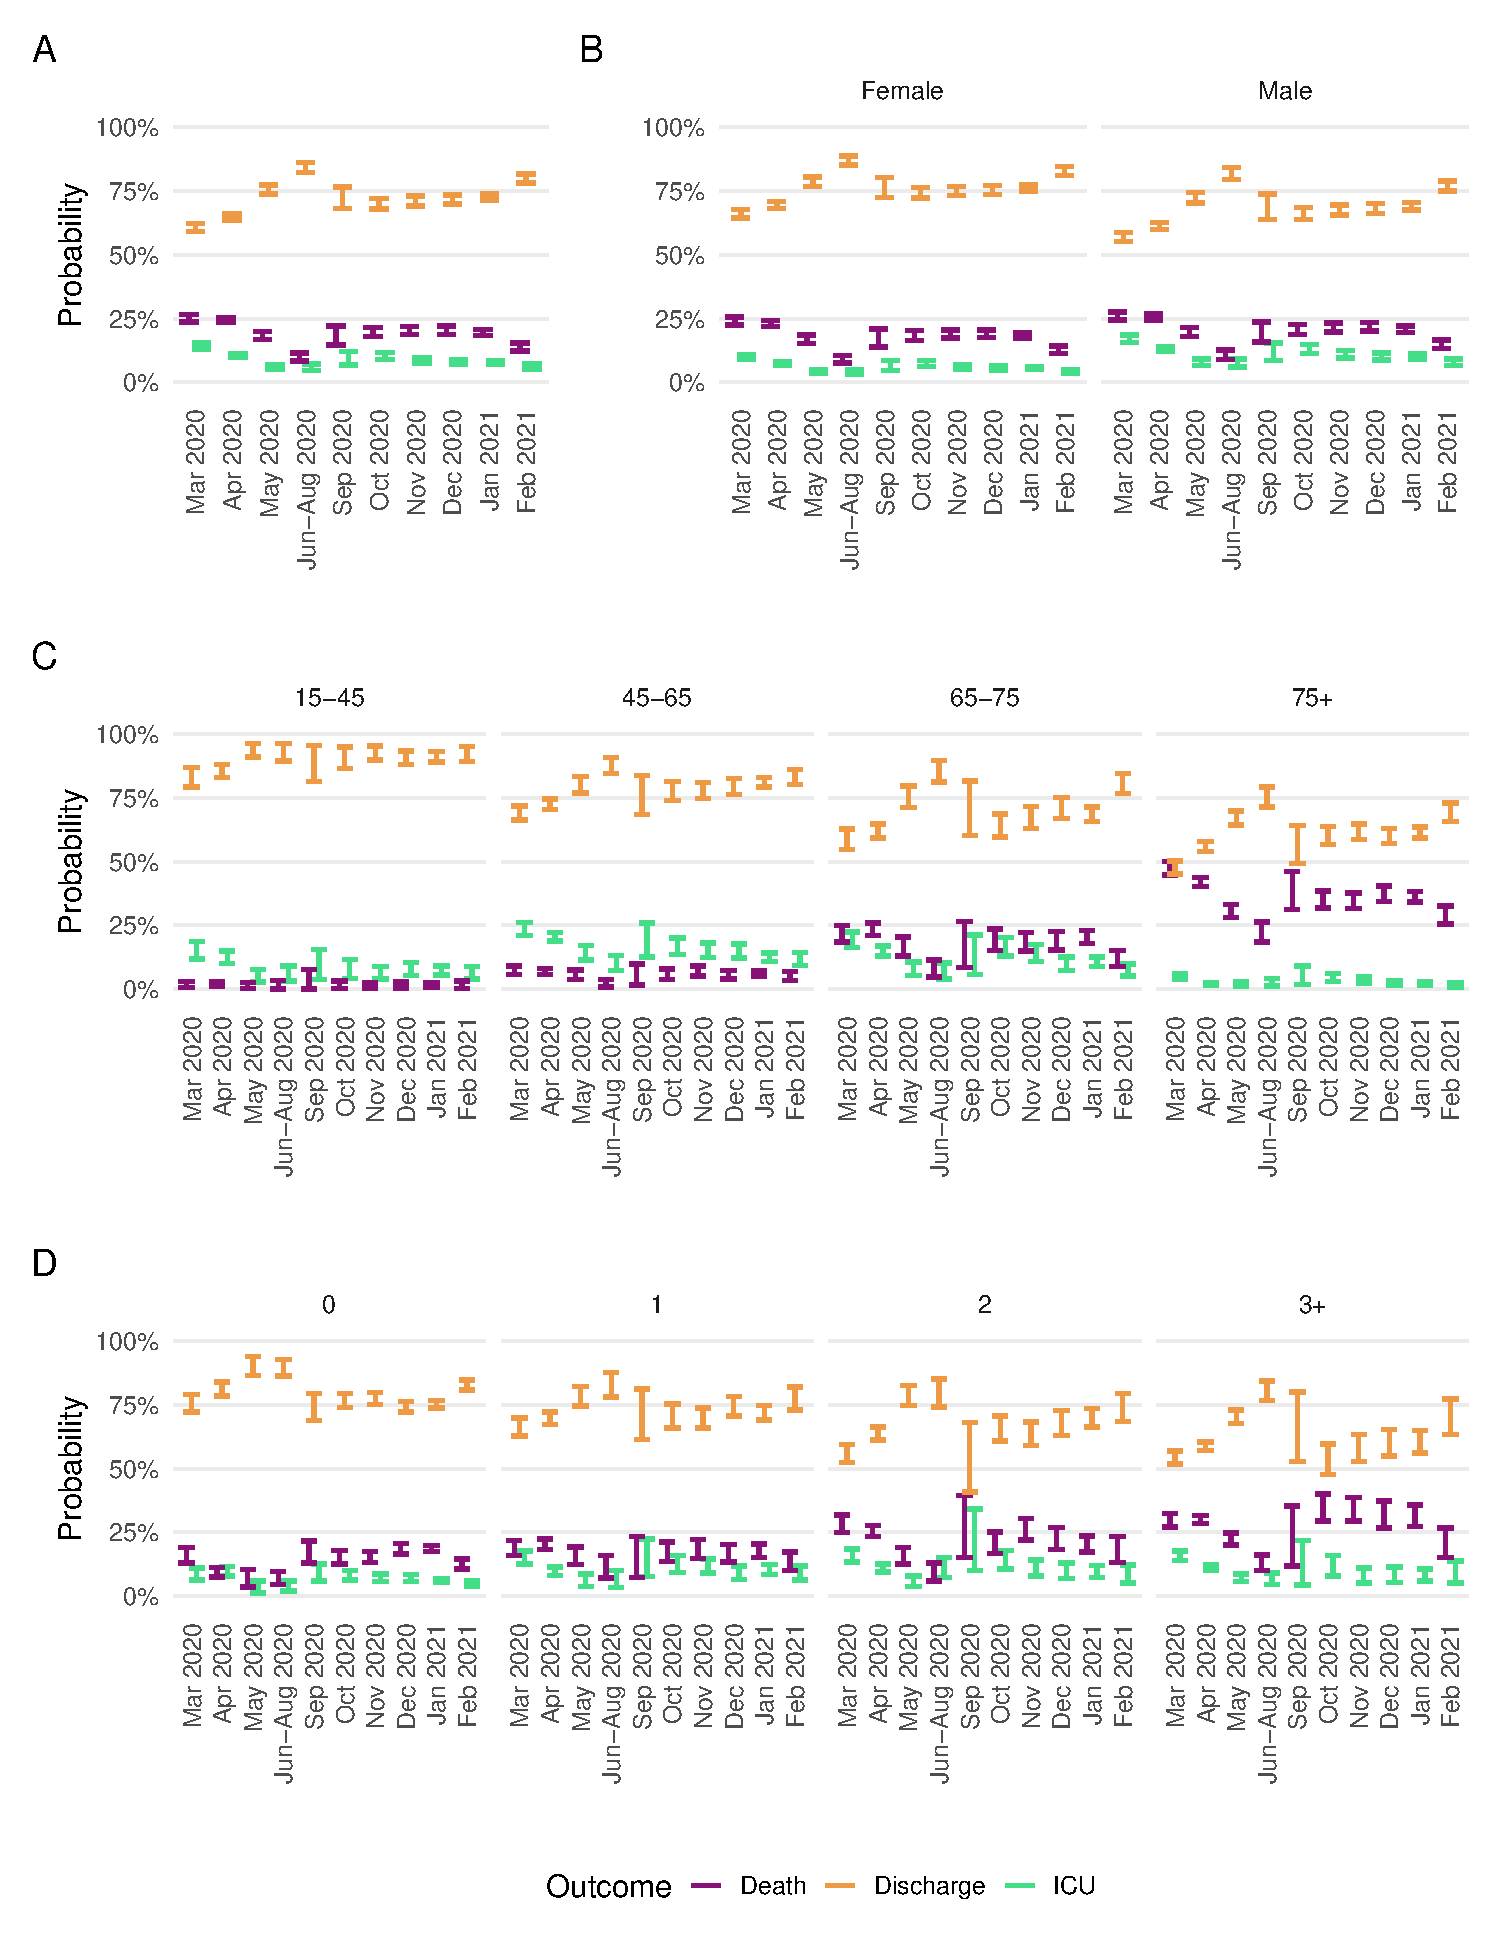
\includegraphics[width=\textwidth]{sari_event_prob.pdf}
    \caption[Probability of next event following hospital admission in SARI-Watch data estimated using multi-state mixture model, March 2020 to February 2021]{Probability of next event and 95\% CI following hospital admission in SARI-Watch data estimated using multi-state mixture model, March 2020 to February 2021. By month of admission (panel A), sex (panel B), age group (panel C), and number of comorbidities (panel D).}\label{fig:sari-event-prob}
\end{figure}

Figure~\ref{fig:sari-med-time}, panels A--D, show estimated median times from hospital admission to next event by month of admission, sex, age group, and number of comorbidities. Time to ICU admission remained low throughout the period, at around \var{sari_los_hosp_icu} days after hospital admission. Median length of stay in hospital prior to death in non-critical care increased from \var{sari_los_hosp_death_mar} in March 2020 to \var{sari_los_hosp_death_dec} in December 2020, with a similar trend across all subgroups. Meanwhile, median lengths of stay in non-critical care prior to discharge fell from \var{sari_los_hosp_disc_mar} for admissions during March to \var{sari_los_hosp_disc_jun} in June/July/August, but lengthened to \var{sari_los_hosp_disc_dec} by December. Stays in non-critical care prior to discharge were longest for older patients, e.g.\ \var{sari_los_hosp_disc_mar_75} in March 2020 among those aged 75+ compared to \var{sari_los_hosp_disc_mar_1545} for those aged 15--45.

Corresponding probabilities and lengths of stay following ICU admission are included in Appendix~\ref{appendix:sari-icu}.

\begin{figure}[htbp!]
    \centering
    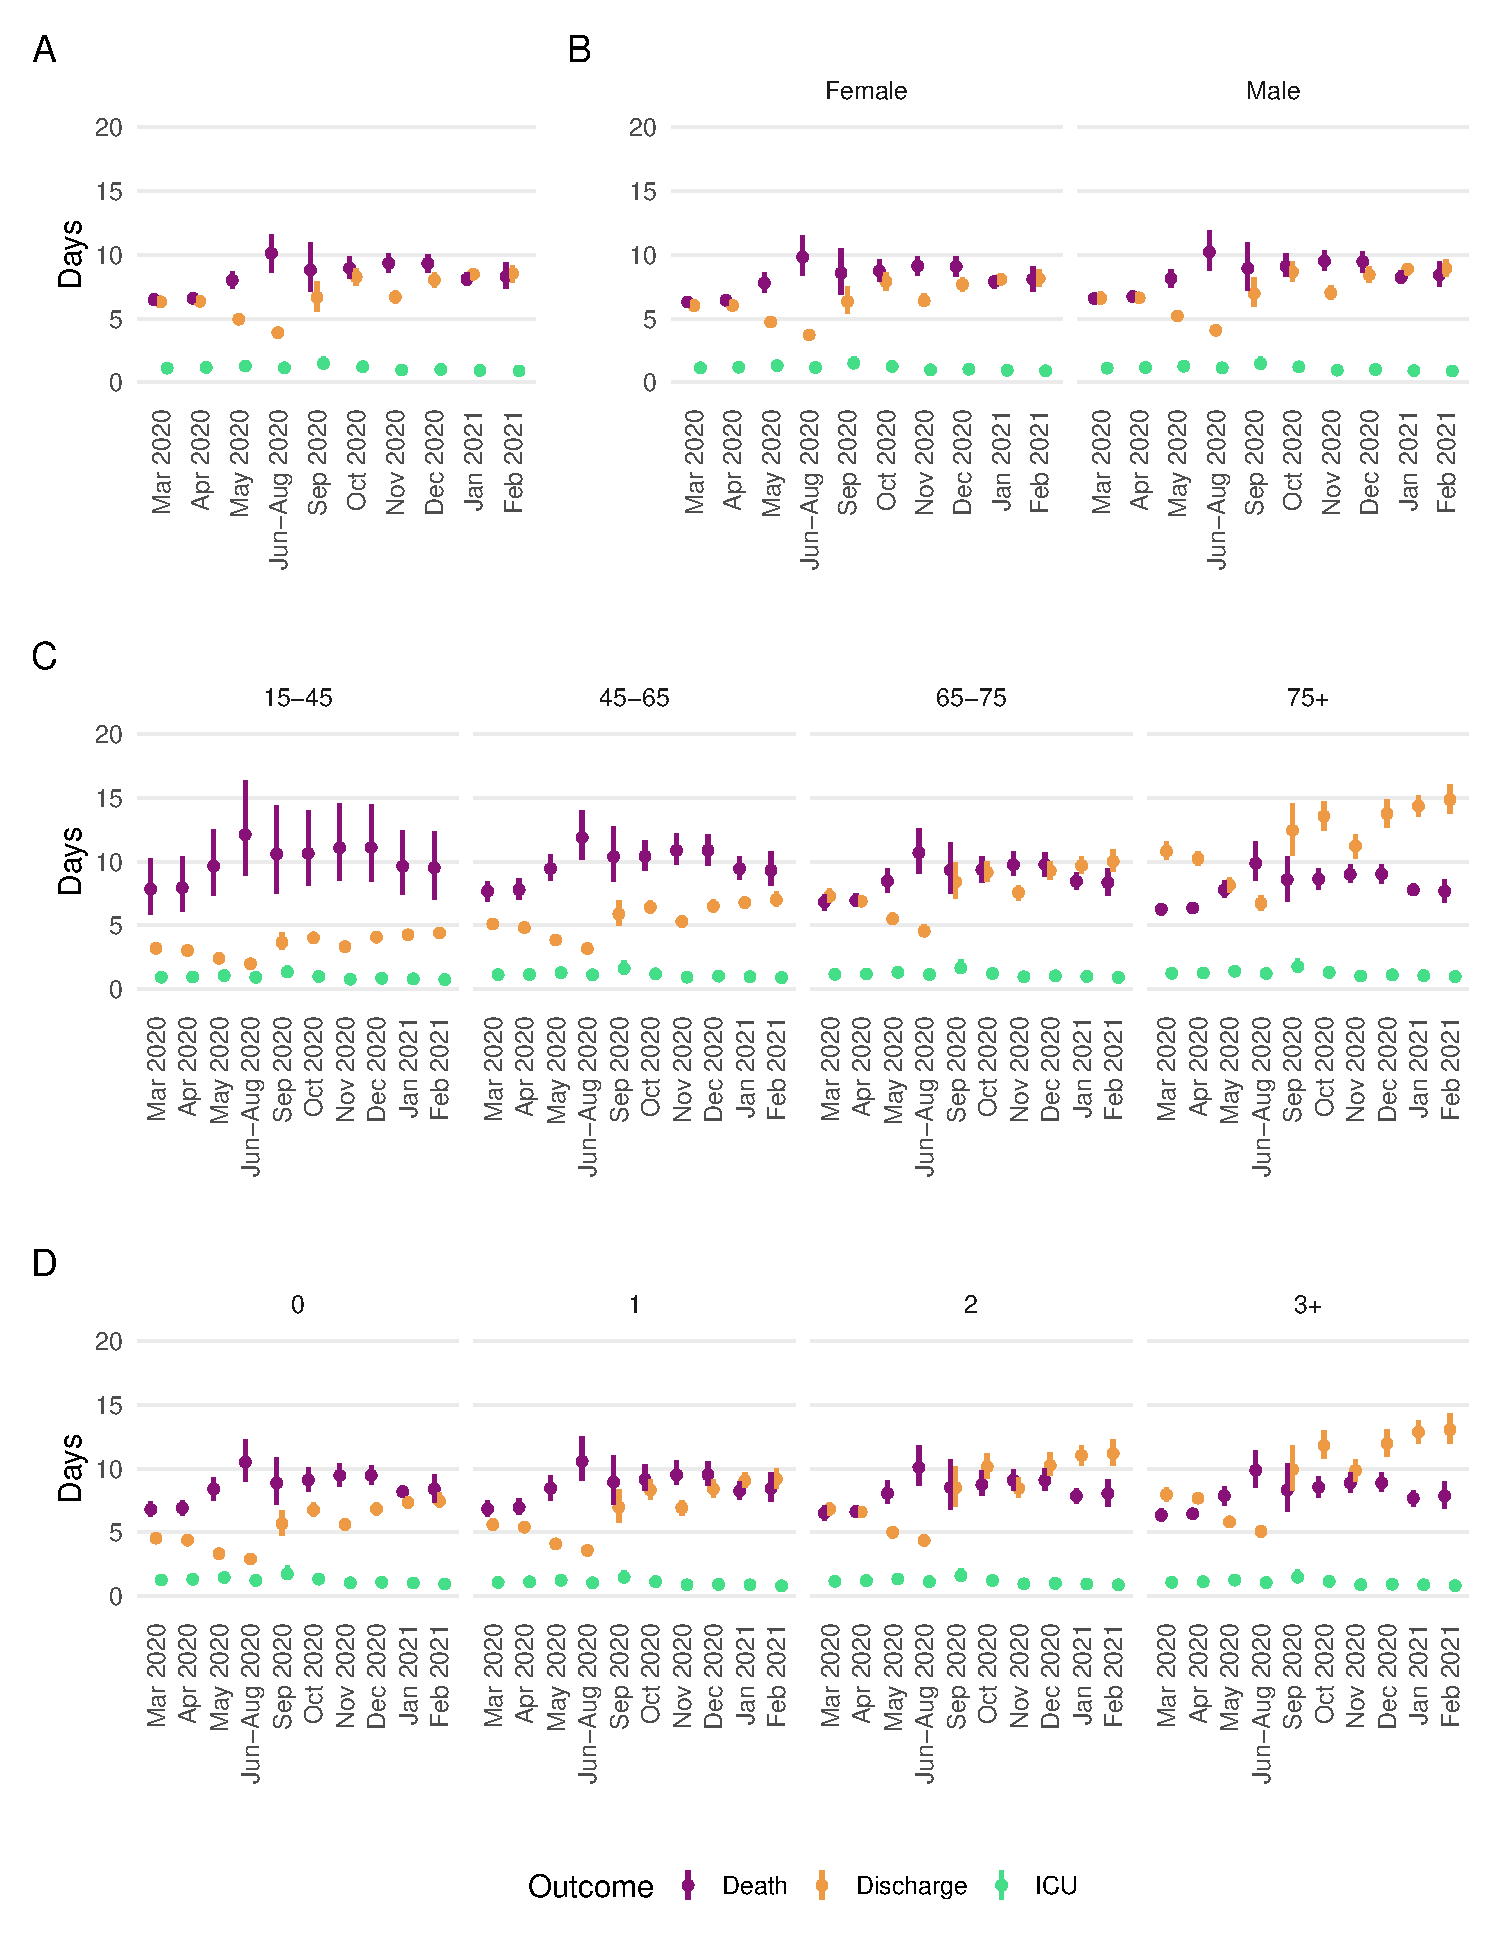
\includegraphics[width=\textwidth]{sari_med_time.pdf}
    \caption[Median time to event following hospital admission in SARI-Watch data estimated using multi-state mixture model, March 2020 to February 2021]{Median time to event and 95\% CI following hospital admission in SARI-Watch data estimated using multi-state mixture model, March 2020 to February 2021. By month of admission (panel A), sex (panel B), age group (panel C), and number of comorbidities (panel D).}\label{fig:sari-med-time}
\end{figure}

HFR estimates which combine the two sub-models (with and without ICU admission) are shown in Figure~\ref{fig:sari-hfr}. Between March and June-August 2020, HFR reduced from \var{sari_hfr_mar} to \var{sari_hfr_jun}; this was followed by an increase to \var{sari_hfr_dec} for patients admitted in December 2020 and a fall to \var{sari_hfr_feb} by February 2021. Whilst the initial fall in HFR was estimated across all subgroups, the increase in December was estimated particularly in the oldest age group (75+) and those with three or more comorbidities, with estimated HFRs of \var{sari_hfr_dec_age_75} and \var{sari_hfr_dec_comorb_3} for admissions in the final month of 2020, respectively.
\newline

\begin{figure}[htbp!]
    \centering
    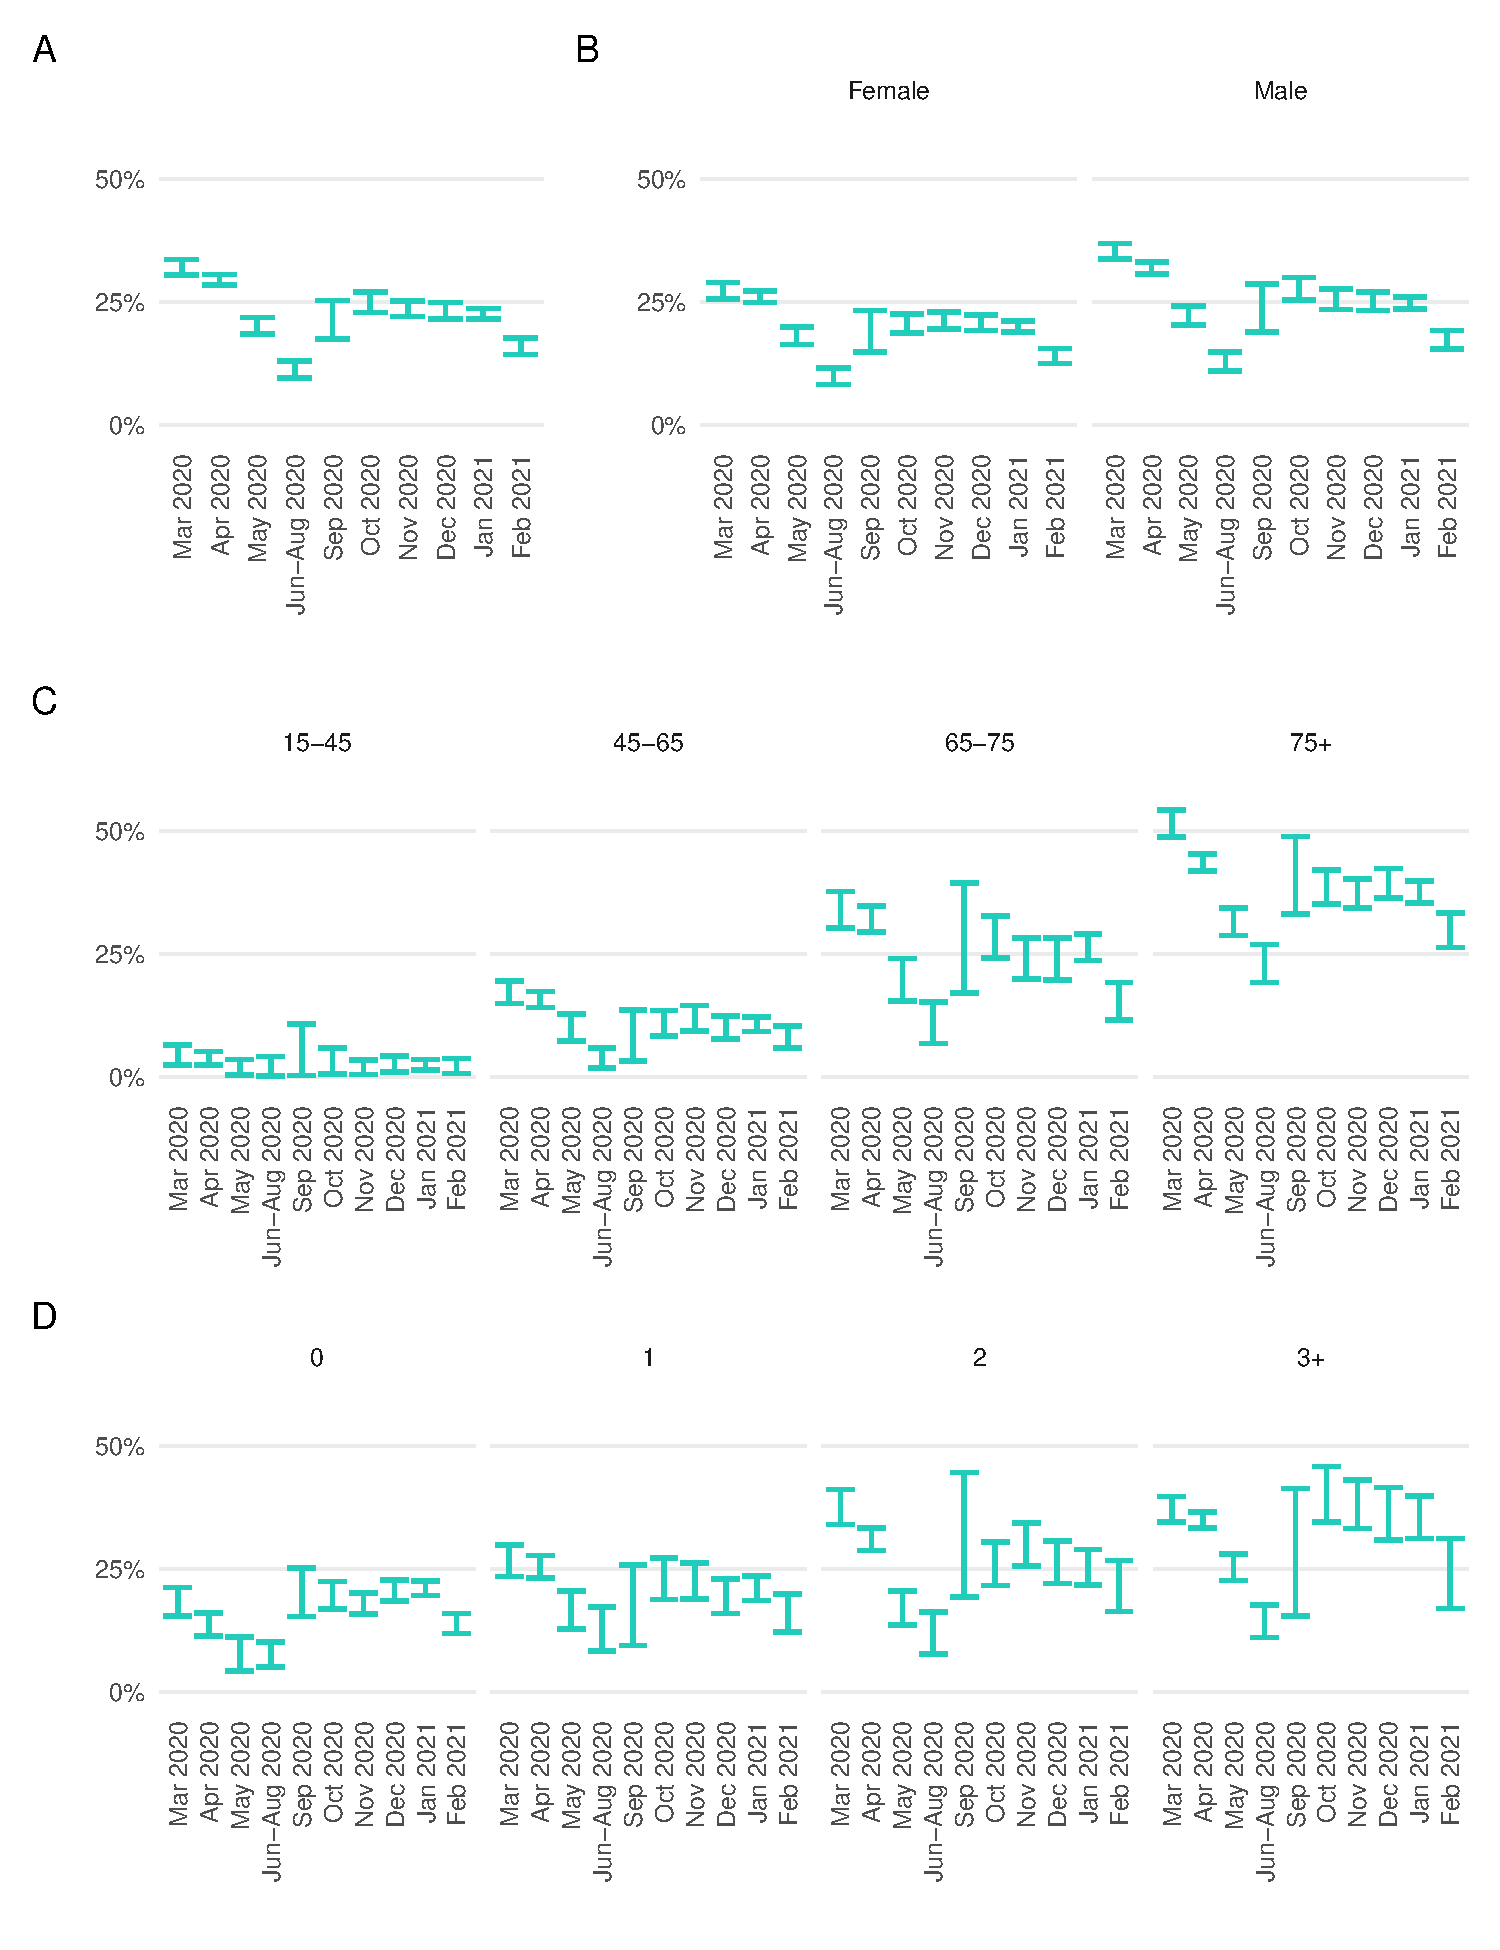
\includegraphics[width=\textwidth]{sari_hfr.pdf}
    \caption[Hospitalised case-fatality risk (HFR) averaged over ICU and non-ICU admission in SARI-Watch data estimated using multi-state mixture model, March 2020 to February 2021]{Hospitalised case-fatality risk (HFR) and 95\% CI averaged over ICU and non-ICU admission in SARI-Watch data, estimated using multi-state mixture model, March 2020 to February 2021. By month of admission (panel A), sex (panel B), age group (panel C), and number of comorbidities (panel D).}\label{fig:sari-hfr}
\end{figure}

\subsubsection{Seasonality}

A somewhat seasonal trend in HFR was observed and the use of a smoothed functions of time to model seasonality in COVID-19 mortality rates was considered, in addition to the categorical month of admission. The Serfling model has been previously implemented to monitor death registrations in European countries~\parencite{Nielsen2013-jh, Serfling1963-ju}. For this model, weekly mortality counts ($w$) were modelled as a function of calendar time, with sine and cosine terms to represent seasonality:
%
\[
    \sin(2\pi \frac{w}{52}), \enspace
    \cos(2\pi \frac{w}{52})
\]

Figure~\ref{fig:cyclic-regression} shows the result of including trigonometric functions of the week of admission as covariates on the probabilities $\pi_{r,s}$, and distribution parameters $\theta_{r,s}$, with comparison to the categorical estimates. HFR estimates based in the trigonometric functions were similar throughout the first half of 2020, but there was a lack of fit to the data in later months.

\begin{figure}[htbp!]
    \centering
    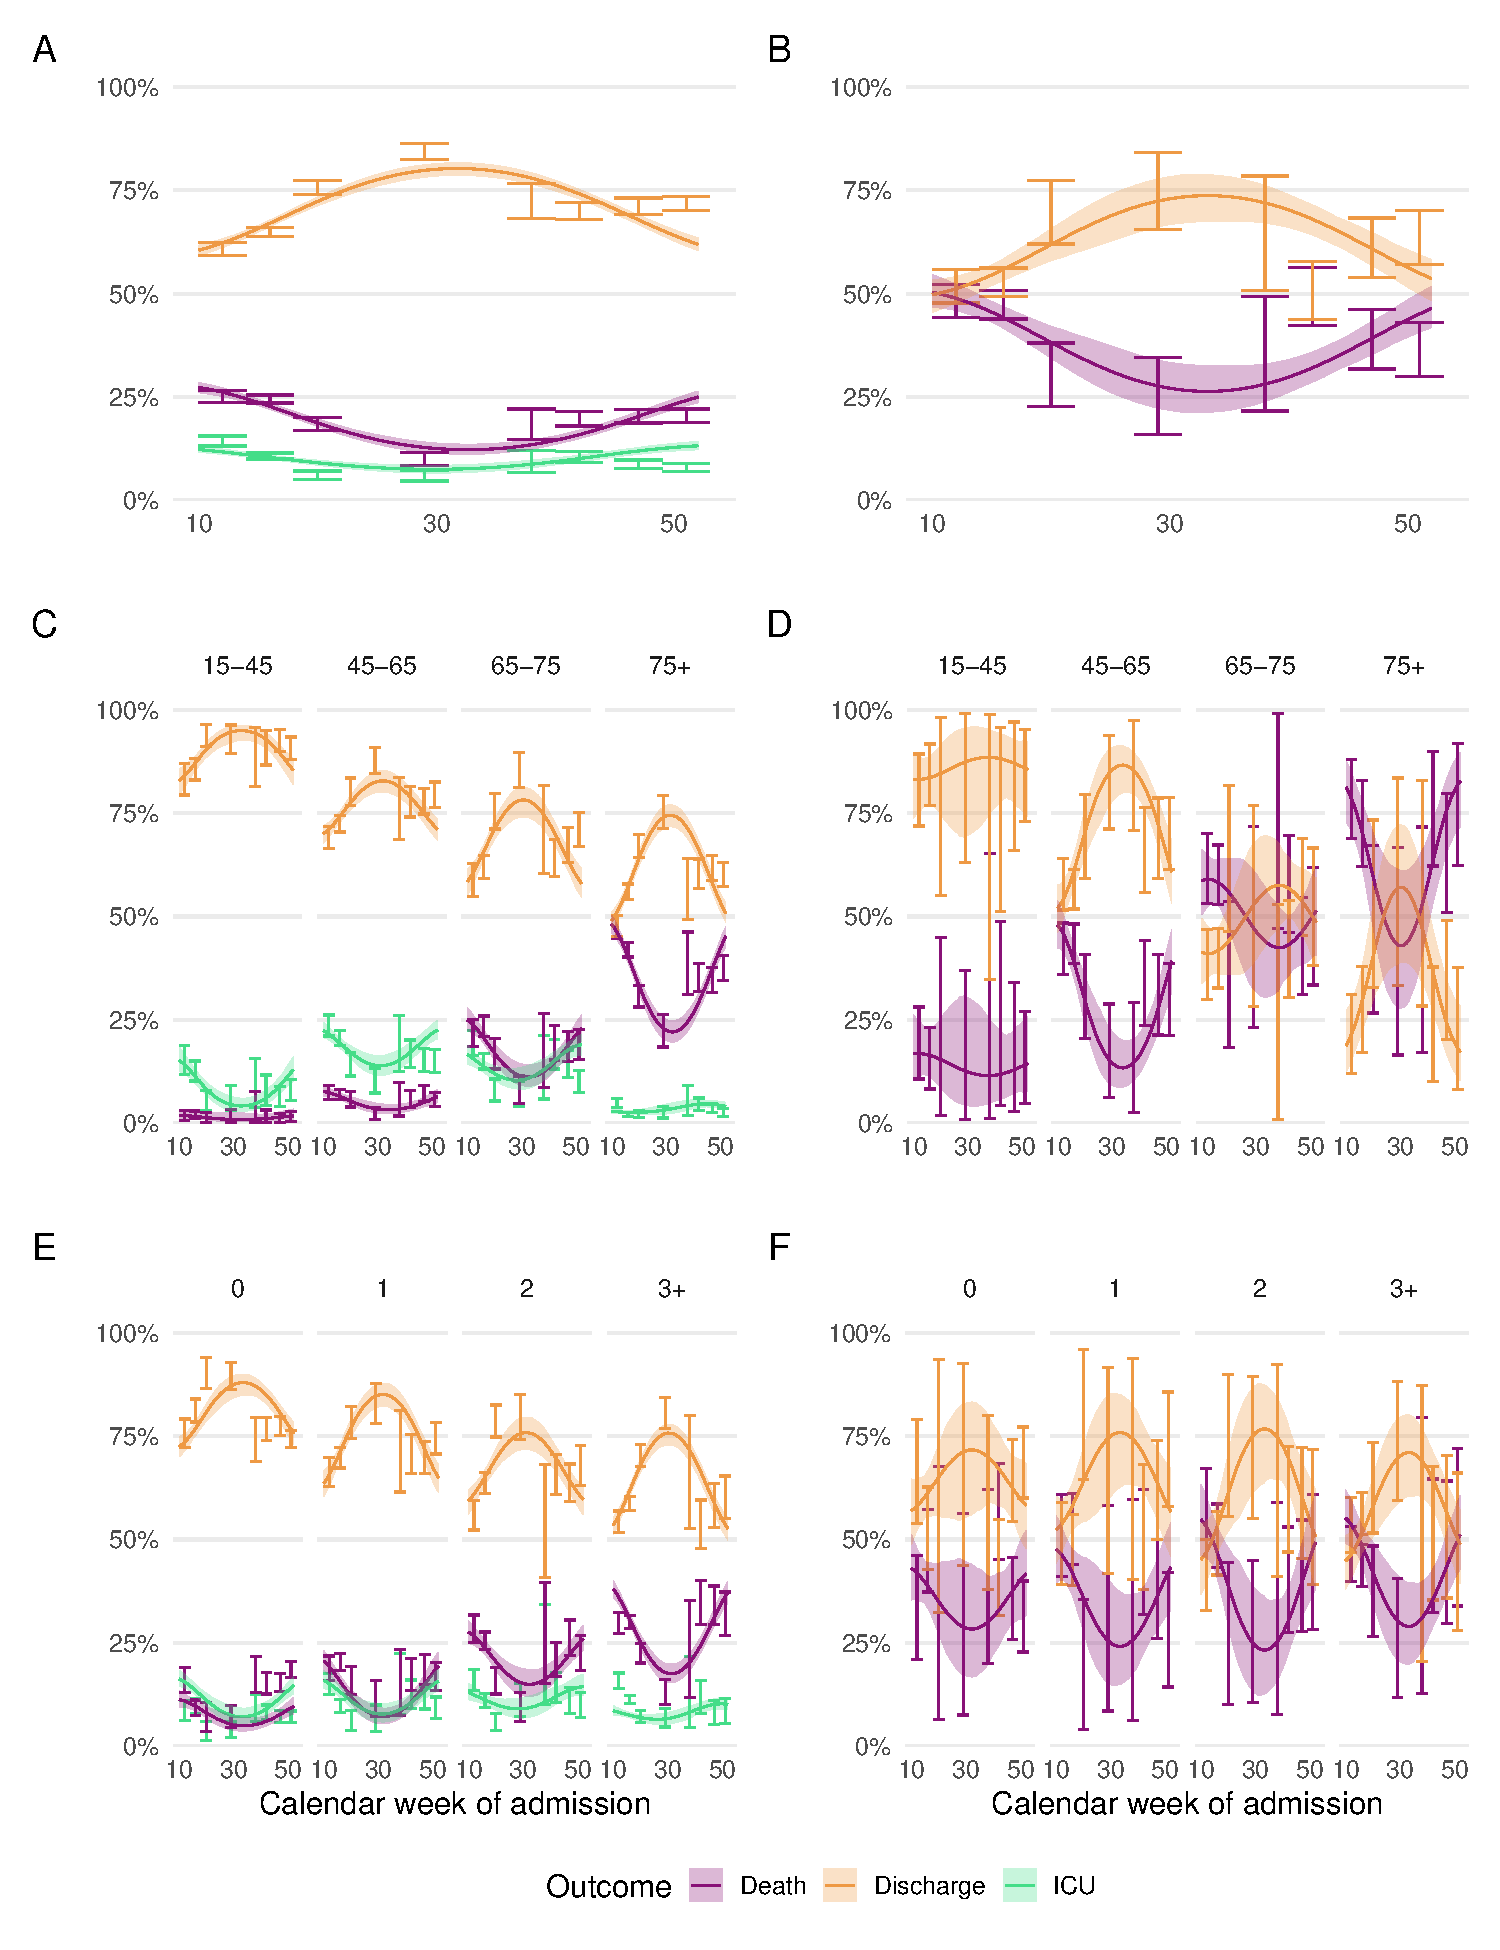
\includegraphics[width=\textwidth]{sari_weekly_prob.pdf}
    \caption[Outcome probabilities for hospital and ICU mixture models with categorical month and trigonometric week parameters in SARI-Watch data, March 2020 to February 2021]{Outcome probabilities and 95\% CI for hospital and ICU mixture models in SARI-Watch data, March 2020 to February 2021. By month and week (panels A and B), including age (panels C and D), and comorbidity (panels E and F). Lines and shaded regions are trigonometric estimates, line ranges are categorical estimates.}\label{fig:cyclic-regression}
\end{figure}

\subsection{Discussion}

This analysis of COVID-19 hospital surveillance data provides a comprehensive assessment of hospital severity over the first two waves of the pandemic, covering the pre-vaccine period in England. Risks of severe events and lengths of stay in hospital were found to vary over time and according to baseline characteristics.

The hospitalised case-fatality risk fell during the first wave of the pandemic (March to June 2020), with a resurgence estimated across all subgroups in autumn/winter 2020/21, particularly for older patients and those presenting with multiple comorbidities. Lengths of stay in hospital for COVID-19 patients, meanwhile, increased throughout this period, and were longer for older patients and those with multimorbidity.

The estimated decline in hospitalised mortality during the initial months of the COVID-19 pandemic in England supports the findings of~\cite{Docherty2020-mr} and~\cite{Gray2021-xk}, who estimated reductions in HFR from 35\% to 15\% and from 52\% to 17\%, respectively, during the first wave. These, and other studies, have reported the same association between COVID-19 severity, age, gender, ethnicity, and comorbidity explored in this analysis~\parencite{Williamson2020-xk, Navaratnam2021-ak}.

By extending the follow-up period through to the end of winter 2021, and accounting for competing risks, longer-term trends in the risks of ICU admission, death, and hospital discharge, and lengths of stay for both critical and non-critical care patients could be estimated. The mortality trends among intensive care patients matched an increase in mortality during autumn 2020 reported by the~\cite{Intensive-Care-National-Audit-and-Research-Centre2021-vs}.

The lack of fit when incorporating seasonality may indicate that assumptions about the `cyclical' nature of the distributions were too strong. Future work might consider the use of splines to define a smooth function of time with fewer assumptions.

Improved patient management and containment of COVID-19 via lockdown restrictions likely contributed to the reduction in mortality during the first wave of infection in England~\parencite{Recovery-Collaborative-Group2020-gi, Bamford2020-vh, Davies2020-kk}. Subsequent changes in case-mix, easing of national restrictions, new variants, and changes in critical care admission criteria may have contributed to the resurgence in hospital pressures during autumn and winter 2020/21 reported by~\cite{Roxby2020-vy}, and the estimated increase in mortality~\parencite{National_Health_Service2020-ue}. Indeed, the severity of the B.1.1.7 VOC-202012/01 (Alpha) variant, which emerged in in December 2020, was likely higher than the wild type variant~\parencite{Davies2021-ua, Scientific_Advisory_Group_for_Emergencies2021-wj, Nyberg2021-cr}.

The substantial drop in HFR observed at the end of the study period coincided with the receipt of second vaccine doses by those most at risk, an intervention which was found to be highly effective in reducing COVID-19 mortality~\parencite{Lopez_Bernal2021-gt}. Whilst additional SARI-Watch data covering the post-vaccination period were not available for this analysis, the effect of vaccination on severity is further explored in the next section.

Interim estimates of HFR using these methods have informed several of the expert scientific panels mobilised during the initial months of the COVID-19 pandemic, including SPI-M, SAGE, and the New and Emerging Respiratory Virus Threats Advisory Group (NERVTAG)~\parencite{Govuk2020-re, Govuk2020-ga, Govuk2020-lb}. The application of competing risks mixture models to COVID-19 data presented here contributed to a joint publication~\parencite{Jackson2022-lt}, and additional results from this analysis have been made available as a pre-print~\parencite{Kirwan2021-sw}.

\subsubsection{Biases and limitations}

The data used for this analysis were collected from a subset of sentinel clinics, representing only 31 out of >200 NHS trusts in England. Whilst initially chosen to be geographically representative, trusts in SARI-Watch chose whether to continue sentinel reporting during the pandemic, with certain regions being under-represented in the dataset (e.g.\ London) which could bias the estimates of HFR\@. To assess the impact of this bias covariate effects were compared with the population-level estimates of death and hospital admission of~\cite{Williamson2020-xk}, with the lower HFR in this study likely due to the lower representation in London. The next section addresses this bias by considering HFR among all NHS trusts, rather than a subset.

Another limitation of the sentinel reporting was the smaller number of patient records than were available for other comparable studies~\parencite{Ferrando-Vivas2021-ut, Docherty2021-es}. This increased the degree of uncertainty in the estimates, particularly among BAME patient groups, and limited analyses to only two covariates for the most part (month of admission plus one demographic factor). The extent to which interactions between covariates could be explored was therefore limited, and these associations must be interpreted carefully due to the potential for confounding.

Whilst covariate information was generally well completed, with validation via linkage to the HES dataset, outcome information was more likely to be missing towards the end of the study. Right censoring and linkage to the UKHSA mortality dataset helped to mitigate this missing information bias, with no obvious systematic bias in reporting.

Finally, the estimated trends in hospital outcomes may have been influenced by epidemic phase. As described in Section~\ref{sec:observational-bias}, a sensitivity analysis can be used to assess epidemic phase bias. This analysis should condition on the symptom onset date, rather than the hospital admission date, since there are several factors other than epidemic phase which may influence the time from infection to hospital admission. Whilst symptoms data were unavailable in SARI-Watch, this bias will be investigated among all hospitalised individuals in the following section.

\section{Post-vaccine hospitalised severity}

The extensive vaccination campaign in England during 2021 led to a marked reduction in the number of individuals being hospitalised, and in the overall risk of mortality~\parencite{Lopez_Bernal2021-gt, Thygesen2021-kg, UK_Health_Security_Agency2021-gw}. Nonetheless, individuals continue to experience COVID-19 infection severe enough to require hospitalisation. In 2021 there was little information about prognosis following hospital admission in the context of widespread vaccination, or how this might be related to hospital load.

In this section I investigate trends in mortality among all people hospitalised with community-onset COVID-19 in England over the first three waves (two years) of the pandemic, and how these trends have varied according to vaccination status, hospital load, and other factors. Relative and absolute risks of hospitalised fatality and lengths of stay in hospital by outcome are estimated using Aalen-Johansen estimators and Fine-Grey proportional hazards regression.

\subsection{Data}

The SUS dataset contains well-completed, accurate information on all hospitalisations for COVID-19 in England. For this analysis, data on all adults (aged 15+) with community-acquired COVID-19 (defined as a positive test for COVID-19 within -14 to 1 days of hospital admission), admitted to hospital in England for COVID-19 or another non-injury related condition during the first two years of the pandemic (March 2020 to April 2022) were considered. Data were extracted in August 2022, allowing four months of follow-up to minimise the impact of lags in data reporting.

Since records are only entered into SUS upon completion of a hospital stay (i.e.\ at the point of discharge from hospital, or death) these were routinely supplemented with information on individuals still in hospital though linkage to ECDS, as well as data on vaccination and PCR testing for COVID-19, as described in Section~\ref{sec:covid-hosp-data}. Among those with completed hospital episodes, 77\% were admitted via emergency care.

\subsubsection{Covariates}

Covariates in the linked dataset included vaccination status (as shown in Figure~\ref{fig:sus_vaccine_month}), date of hospital admission, age group, region of residence, Charlson Comorbidity Index (CCI)\parencite{Charlson1987-nz}, ethnicity, sex, and index of multiple deprivation (IMD)\nomenclature[z]{IMD}{Index of multiple deprivation} quintile. A hospital load measure was derived from the number of COVID-19 admissions at an NHS trust within the 7 days around admission (3 before, same day, and 3 after). Hospital load was calculated as a proportion of the busiest 7-day period at that trust, grouped into: 0--20\%, 20--40\%, 40--60\%, 60--80\%, 80--90\%, and 90--100\%.

\begin{figure}[htbp!]
    \centering
    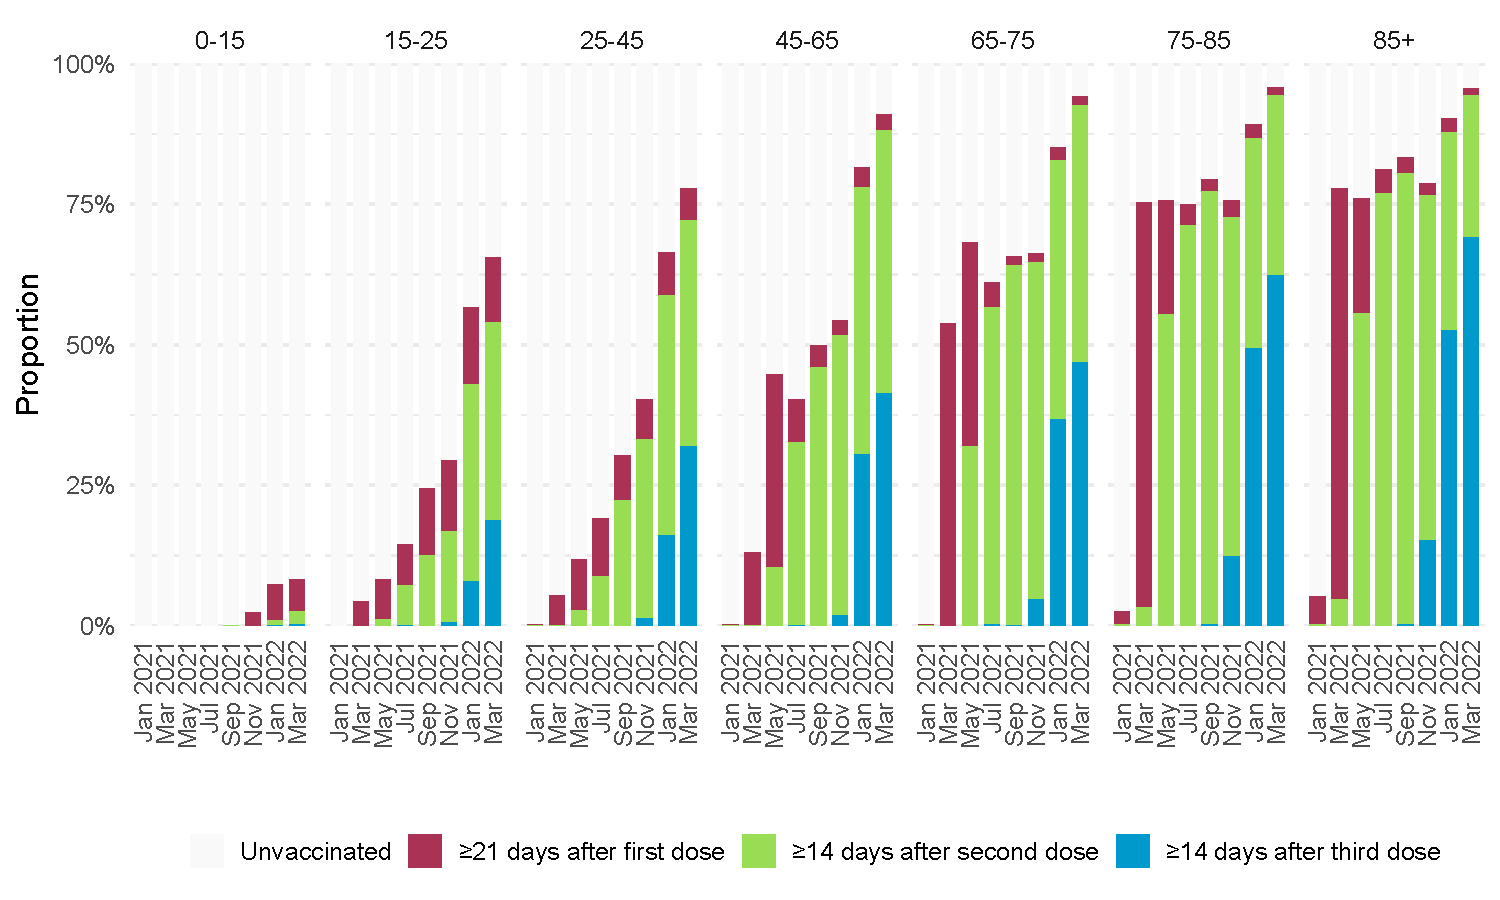
\includegraphics[width=\textwidth]{sus_vaccine_month.pdf}
    \caption[Vaccination status of hospitalised individuals in SUS data, by month of admission and age group, March 2020 to April 2022]{Vaccination status of hospitalised individuals in SUS data, by month of admission and age group, March 2020 to April 2022.}\label{fig:sus_vaccine_month}
\end{figure}

The number of reported admissions were compared with the NHS weekly COVID-19 admissions data to ensure data were representative~\parencite{NHS-England2022-bh}. Hospital-onset COVID-19 (i.e.\ infection occurring in hospital) cases were excluded:\ those who acquired COVID-19 infection in hospital during the study period ($n$ = 209,139) tended to be older and have longer lengths of stay than the community-onset cases considered in this study, with a greater proportion remaining in hospital post-90 days (Table~\ref{tab:sus_characteristics}). Hospital stays for these individuals may be influenced by conditions other than COVID-19, as described by~\cite{Bhattacharya2021-wq}.

\subsection{Multi-state model}

Two competing risks survival models (Section~\ref{sec:cr-models}) were applied to the SUS data to investigate the competing risks of death and discharge following hospital admission. Given the lack of information about ICU admissions in SUS, these risks are averaged over whether the admission included an ICU stay or not.

Aalen-Johansen cumulative incidence estimation was used to obtain estimates of cumulative HFR and median lengths of stay in hospital for specific sub-sets of the population, unadjusted for other factors. Median lengths of stay were the weighted medians from the Aalen-Johansen estimate with weighted ties (see Section~\ref{sec:weighted-median} for details).

Stratified Fine-Gray competing risk proportional hazards regression with adjustment for confounders was used to estimate the association of each risk factor with the cumulative incidence of mortality within 90-days of hospitalisation with COVID-19 (i.e.\ hospitalised fatality). The proportional hazards assumption was checked for each covariate, and stratification used for confounders with non-proportional hazards.

\subsubsection{Stratification}

For the regression on month of admission, stratification was by age group, region of residence and vaccination status, with regression adjustment on sex, ethnicity, IMD quintile and CCI\@. For the regression on vaccination status, stratification was by age group, region of residence and month of hospital admission, with regression adjustment on sex, ethnicity, IMD quintile and CCI\@.

\subsubsection{Censoring}

To focus these analyses on outcomes following COVID-19 admission, and for consistency with the previous analysis, a pragmatic cut-off of 90 days from first positive specimen date was chosen and only those hospital outcomes (death or discharge) occurring within this cut-off were included. All records with outcomes occurring beyond 90 days ($n$ = 656) were right-censored at 90 days, while individuals who remained in hospital at the date of data extraction ($n$ = 1019) were right-censored at the shorter of this date or 90 days.

Linkage to the UKHSA deaths data enabled post-hospital discharge deaths to be identified. To better account for palliative discharge, deaths occurring within 14 days of discharge from hospital ($n$ = 15,523, 19.1\% of all deaths observed) were classified as deaths rather than discharges, and the date of death used as the outcome date.

\subsubsection{Consistency in model estimates}

Figure~\ref{fig:fg_aj_comparison} demonstrates the high degree of agreement between the Aalen-Johansen and Fine-Gray model cumulative fatality estimates for selected months over the study period.

\begin{figure}[htbp!]
    \centering
    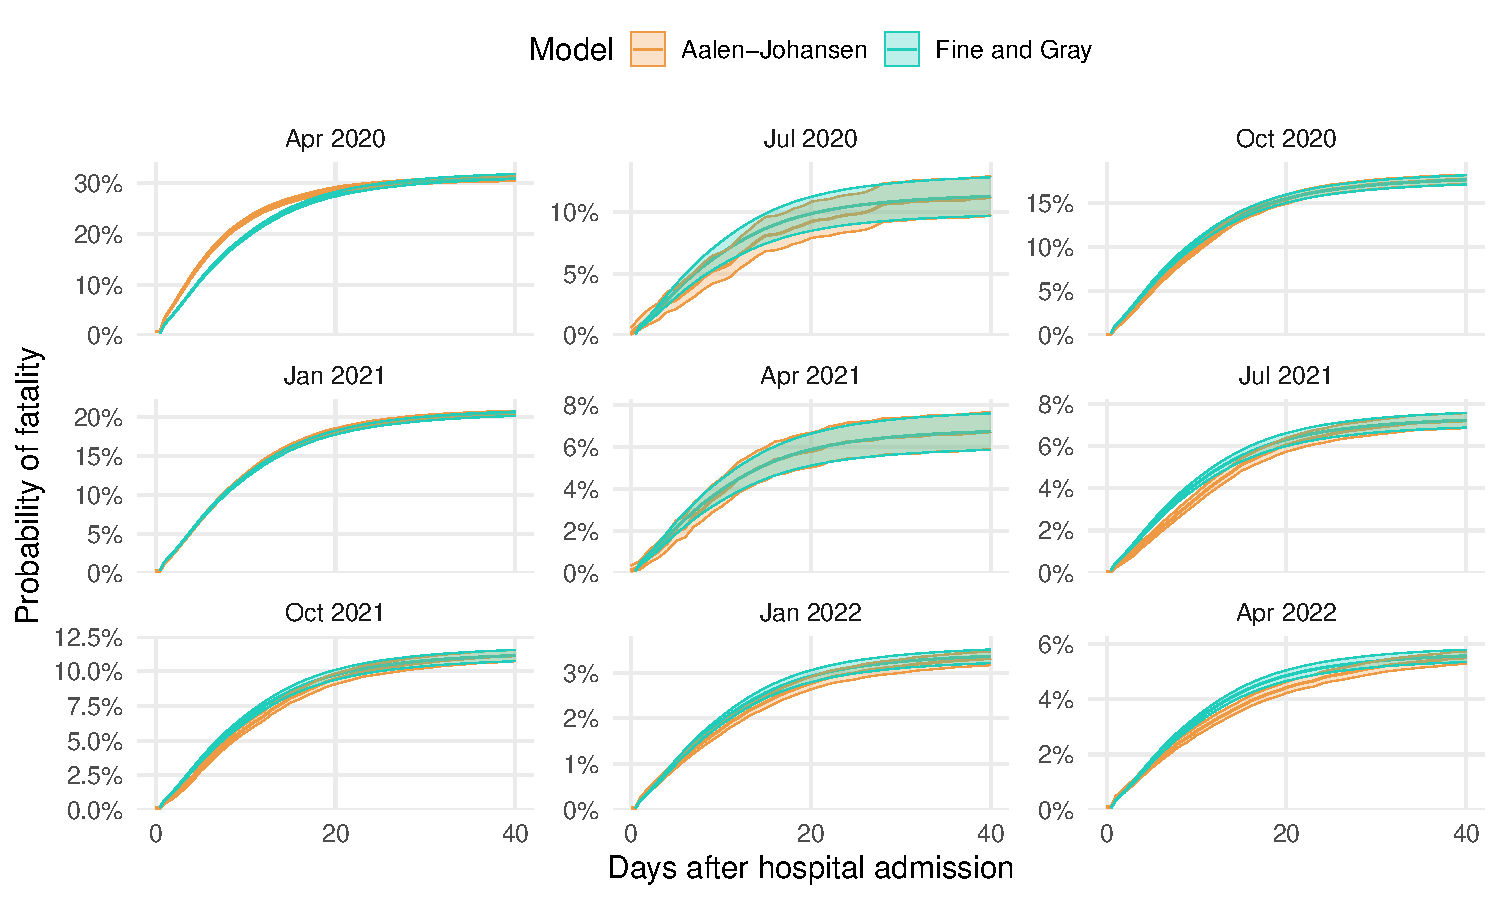
\includegraphics[width=\textwidth]{fg_aj_month_comparison.pdf}
    \caption[Aalen-Johansen and Fine-Gray cumulative fatality estimates for first 60 days following hospital admission in SUS data, March 2020 to April 2022]{Aalen-Johansen and Fine-Gray cumulative fatality estimates for first 60 days following hospital admission in SUS data, with 95\% CI, March 2020 to April 2022}\label{fig:fg_aj_comparison}
\end{figure}

\subsubsection{Epidemic phase bias}

Sensitivity analysis was used to assess the potential effect of epidemic phase bias on the estimated hazard ratios in relative risk analyses. For this analysis the date of symptom onset was conditioned on, rather than the date of hospital admission, to ensure that the sensitivity analysis targeted bias due to epidemic phase, as opposed to any other factors which may influence time from symptom onset to admission.

A time shift of $c = 0,1,2,3,4$ days was added to records with a mortality outcome, where $c$ should represent the mean difference in time from infection to symptom onset date between those who died and those who did not. Based on previous analyses of COVID-19 data this time was not expected to be greater than 4 days~\parencite{Seaman2022-tl}.

\subsubsection{Estimation}

Hospitalised fatality risks and lengths of stay were estimated using the Aalen-Johansen estimator. Sub-distribution hazards were estimated using Fine-Gray proportional hazards regression (see Section~\ref{sec:cr-models}).

Statistical models were implemented using maximum likelihood estimation with the open-source packages \texttt{survival} and \texttt{matrixStats} in \texttt{R}~\parencite{Therneau1999-to, Bengtsson2007-yb, R_Core_Team2020-ca}.

\subsection{Results}

Participant characteristics are shown in Appendix~\ref{tab:sus_characteristics}. Among 590,313 people hospitalised with COVID-19 between March 2020 and April 2022, a total of 81,343 (13.8\%) died, 507,254 (85.9\%) were discharged, and the remaining 1716 (0.3\%) remained in hospital at the date of data extraction and/or were right-censored at 90 days. Compared to all people with PCR-confirmed community-acquired COVID-19 infection, those hospitalised for COVID-19 were older (44\% vs.\ 10\% aged over 65), more likely to live in an area of high deprivation (27\% vs.\ 24\%), and to reside in London (18\% vs.\ 16\%).

Hospitalised fatality risk over the study period is shown in Figure~\ref{fig:hfr-month} panel A. HFR decreased during the first wave of the pandemic from \var{sus_hfr_mar20} in March 2020 to \var{sus_hfr_aug20} in August 2020. In the second wave, HFR peaked at \var{sus_hfr_jan21} in January 2021, but by March 2021 had halved to \var{sus_hfr_mar21}. The peak was smaller again in the third wave, at \var{sus_hfr_oct21} in October 2021.

Patients with an eventual outcome of death generally had longer stays in hospital compared to those who were discharged (Figure~\ref{fig:hfr-month} panel B). Lengths of stay prior to discharge decreased throughout the first wave, from \var{sus_los_disc_mar20} in March 2020 to \var{sus_los_disc_aug20} in August 2020. Over the same time period, lengths of stay prior to death increased from \var{sus_los_death_mar20} to \var{sus_los_death_aug20}. Fluctuation in lengths of stay were estimated throughout the second and third waves, in parallel with trends in HFR\@.

\begin{figure}[htbp!]
    \centering
    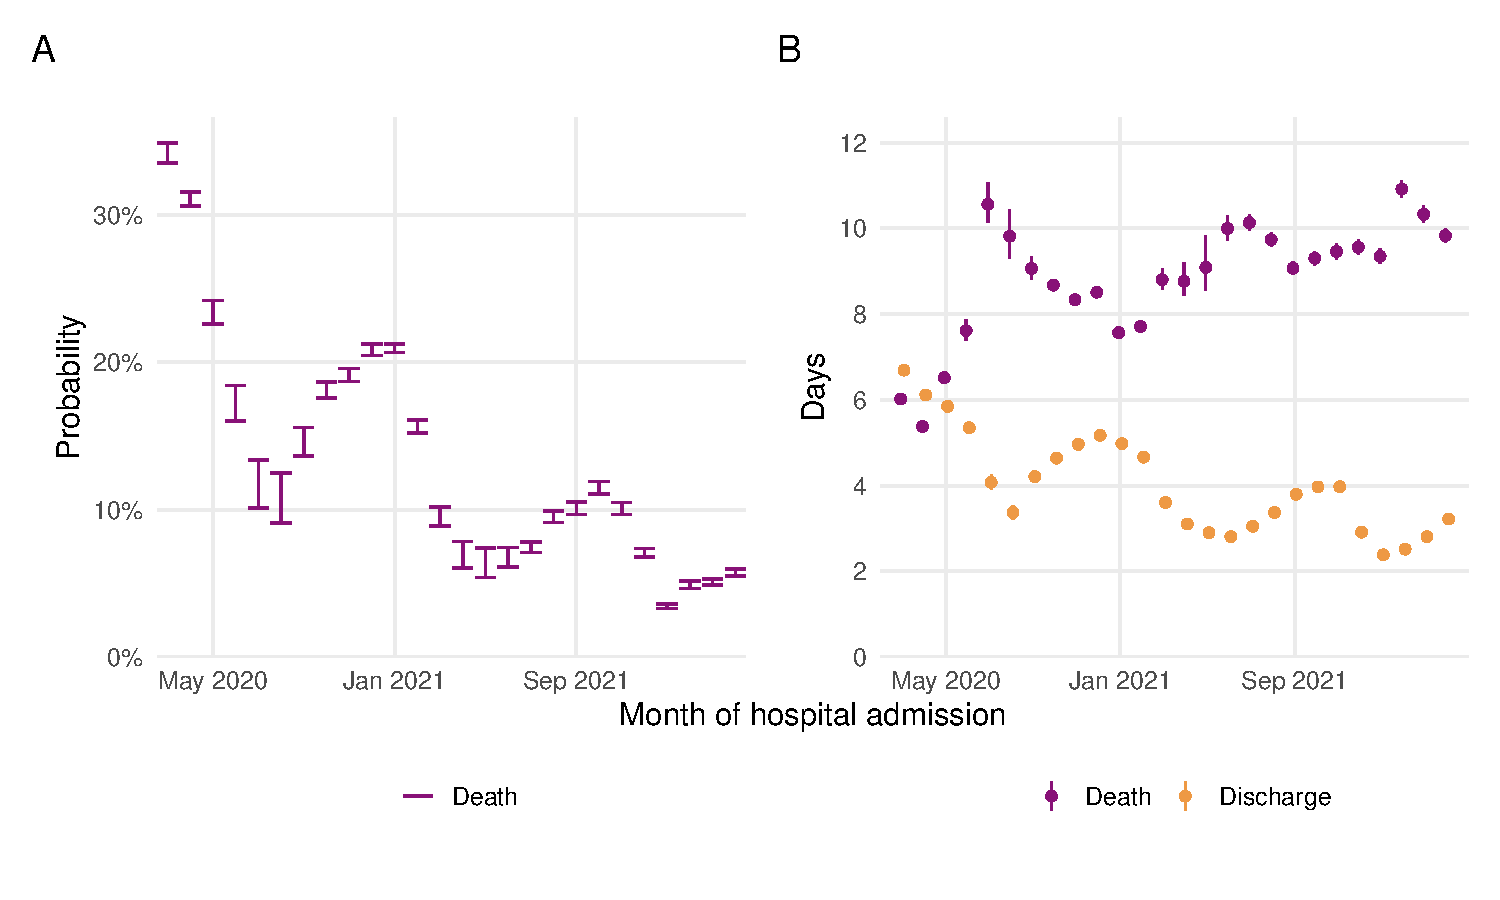
\includegraphics[width=\textwidth]{hfr_month.pdf}
    \caption[Hospitalised fatality risk and median length of stay by month of admission in SUS data, March 2020 to April 2022]{Hospitalised fatality risk (panel A) and median length of stay (panel B) by month of hospital admission. SUS data, with 95\% CI, March 2020 to April 2022. Unadjusted for other covariates.}\label{fig:hfr-month}
\end{figure}

Older individuals and those with multiple co-morbidities were more likely to die or else experienced longer stays prior to discharge (Figures~\ref{fig:hfr-month-age} and~\ref{fig:hfr-month-cci}). Whilst trends are uncertain in months with fewer admissions, those admitted to hospitals experiencing higher load had slightly greater HFR than to those admitted to hospitals with lower activity, e.g.\ during March 2020:\ \var{sus_hfr_load_mar_90} for hospitals at 90--100\% of their peak load, compared to \var{sus_hfr_load_mar_0} for hospitals at 0--20\% of their peak load, and similarly for November 2020:\ \var{sus_hfr_load_nov_90} compared to \var{sus_hfr_load_nov_0} (Figure~\ref{fig:hfr-month-load}).

Figure~\ref{fig:fg-month} shows hazard ratios for hospitalised fatality by month of hospital admission. Controlling for age group, region of residence, vaccine status, sex, ethnicity, IMD quintile, CCI, and hospital load, month of hospital admission remained a significant factor for the prognosis of hospitalised individuals. Compared to June 2020, the hazard for hospitalised fatality was significantly increased during March to May 2020, and September 2020 to February 2021, with much lower HFR estimated at the start of 2022.

\begin{figure}[htbp!]
    \centering
    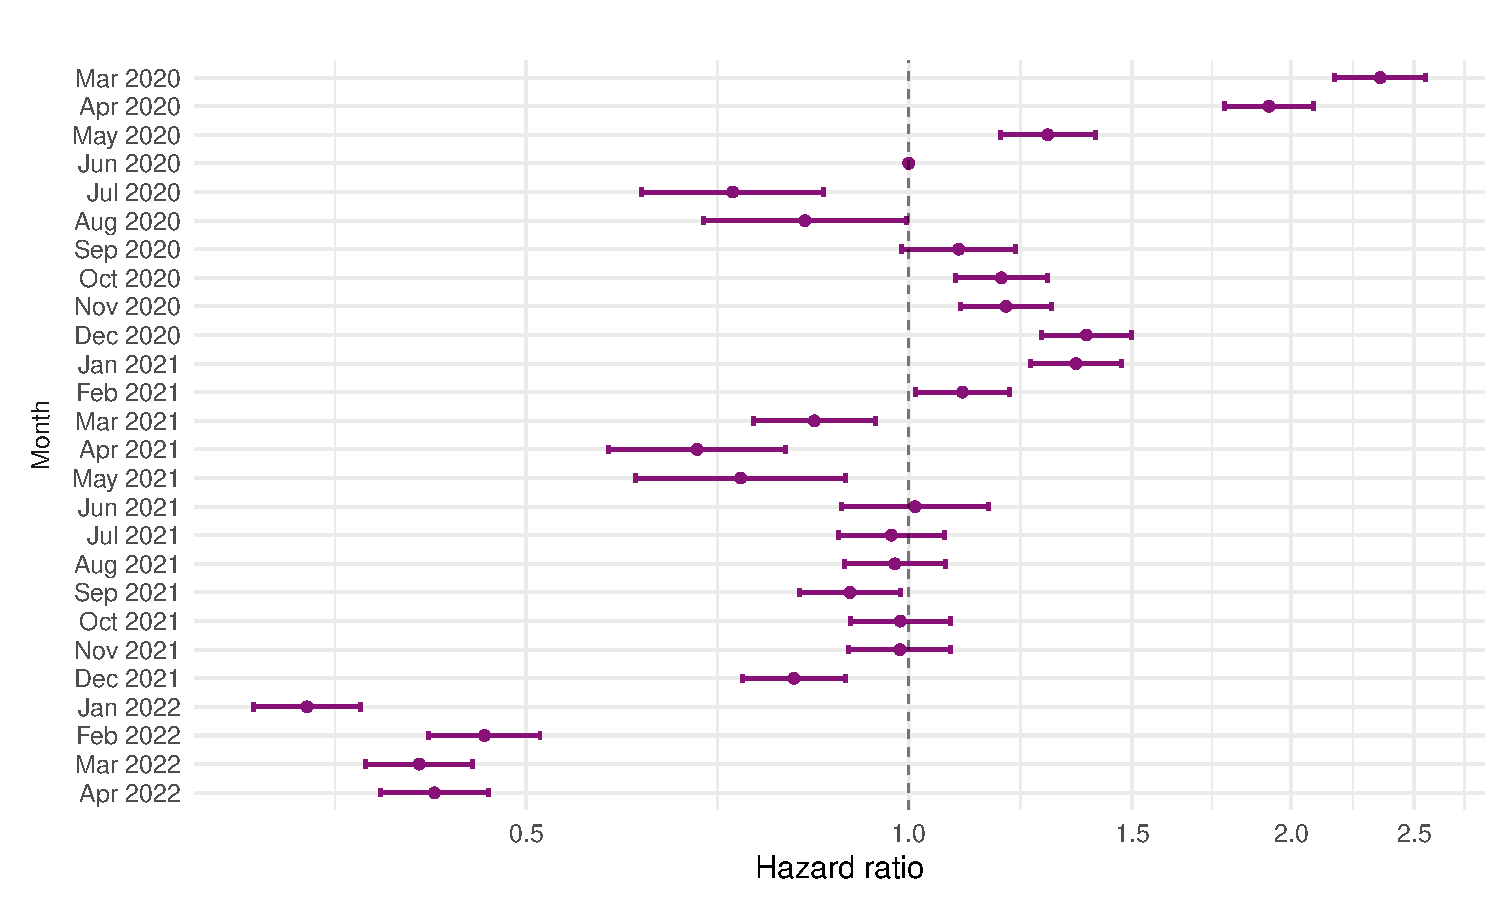
\includegraphics[width=\textwidth]{fg_month.pdf}
    \caption[Hospitalised fatality sub-distribution hazard ratio by month of hospital admission in SUS data, March 2020 to April 2022]{Hospitalised fatality sub-distribution hazard ratio and 95\% CI by month of hospital admission. SUS data, March 2020 to April 2022. Adjusted for:\ age group, region, vaccine status, sex, ethnicity, IMD quintile, CCI, and hospital load. Reference group:\ June 2020.}\label{fig:fg-month}
\end{figure}

Compared to unvaccinated people, controlling for month of hospital admission and the factors mentioned above, the hazard ratio of hospitalised mortality was \var{sus_haz_vac1_36} during the first 3--6 weeks post-first dose vaccination, this increased to \var{sus_haz_vac1_612} for individuals hospitalised during the 6--12 weeks post-first vaccine dose. Hazard ratios were lower following a second vaccine dose, \var{sus_haz_vac2_26} for the first 2--6 weeks post-second vaccine dose, although with similar waning of this protection in the following weeks. A third dose reduced the hazard ratio of hospitalised mortality to \var{sus_haz_vac3_26} in the first 2--6 weeks, and this protection appeared to be sustained for longer (Figure~\ref{fig:fg-vaccine}).

\begin{figure}[htbp!]
    \centering
    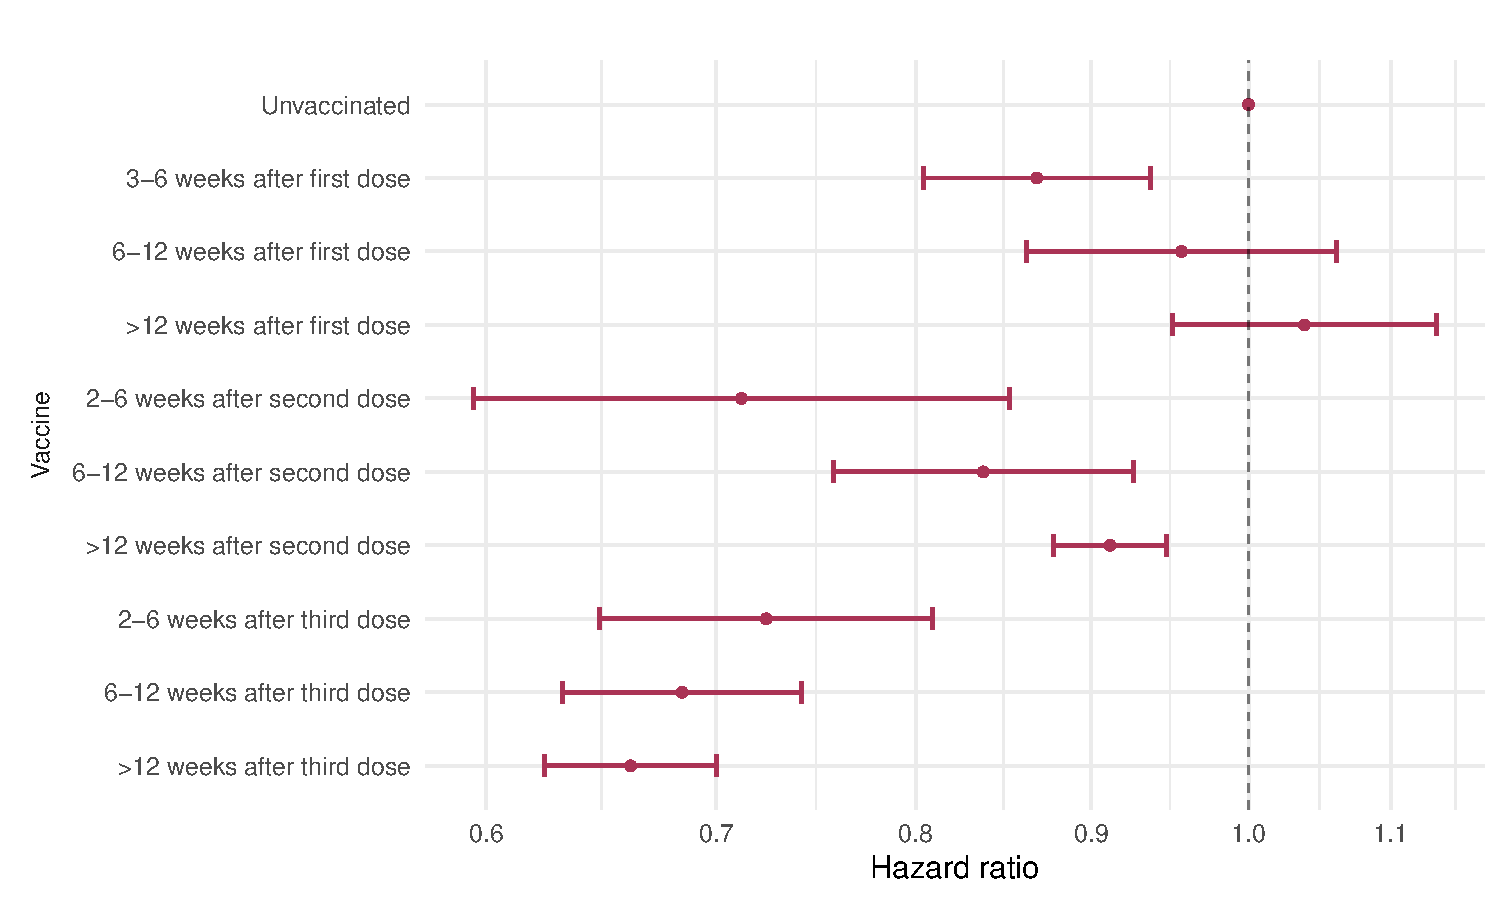
\includegraphics[width=\textwidth]{fg_vaccine.pdf}
    \caption[Hospitalised fatality sub-distribution hazard ratio by vaccine status in SUS data, March 2020 to April 2022]{Hospitalised fatality sub-distribution hazard ratio and 95\% CI by vaccine status. SUS data, March 2020 to April 2022. Adjusted for:\ age group, region, month of admission, sex, ethnicity, IMD quintile, CCI, and hospital load. Reference group:\ Unvaccinated.}\label{fig:fg-vaccine}
\end{figure}

Hazard ratios associated with other patient characteristics are shown Figure~\ref{fig:fg-hazards}. There was an increased hazard of hospitalised fatality among those of Asian ethnicity (\var{sus_haz_asian}) but reduced among those of Black ethnicity (\var{sus_haz_black}) compared to reference category White. Females had a lower hazard of fatality compared to males (hazard ratio \var{sus_haz_female}), and compared to a CCI of 0, those with a higher burden of comorbidity had a greater hazard of hospitalised fatality (hazard ratio \var{sus_haz_cci5} for CCI of 5 and above). Those residing in more deprived quintiles had greater hazards for hospitalised fatality (hazard ratio \var{sus_haz_dep} for the most deprived quintile) compared to a reference of least deprived.

Supplementary Figure~\ref{fig:fg-shift} shows the shift sensitivity analyses by month of symptom onset, adjusted for the same covariates as above. The greatest effect was observed for the March 2020 estimate, which steadily reduced towards 1 following a shift of $c = 1, 2, 3$ or 4 days. The effect in other months was small, with the previously described monthly trends persisting.

\subsection{Discussion}

The prognosis for people hospitalised with COVID-19 in England during the first three waves of the COVID-19 pandemic has varied substantially according to month of admission, case-mix, and vaccination.

In this analysis, greater absolute hospitalised fatality risks were estimated for men, older individuals, and those with multimorbidity, and HFR varied according to ethnicity, month of admission, and hospital load. Lengths of stay in hospital were similarly associated with demographic factors, with median lengths of stay prior to death generally longer than those prior to discharge. In relative risk analyses controlling for all measured confounders, baseline comorbidity burden was the strongest predictor of mortality. Being admitted during a period of high hospital load was also associated with poorer outcomes, but patients received a high standard of care overall, with lockdown measures likely protecting against hospitals becoming excessively overburdened~\parencite{Davies2020-kk}.

A significant reduction in HFR was seen in early 2022, despite a peak in the number of infections in the community (Figure~\ref{fig:pandemic-waves}). This reduction in HFR may be related to the emergence of the Omicron (B.1.1.529) variant in December 2021, which became the dominant circulating variant in January 2022. In complementary analyses of all PCR-confirmed infections in England,~\cite{Nyberg2022-jz} estimated substantially lower risks of hospitalisation and severe events following Omicron infection, as compared to infection with the previous Delta (B.1.617.2) variant.

Estimated risk of hospitalised fatality risk was lower among vaccinated individuals, with the effect most clearly seen in older individuals. For those aged 75 and over, vaccination reduced HFR to approximately the risk of an unvaccinated individual aged 10 years younger. In adjusted estimates, each additional vaccine dose significantly reduced the hazard of hospitalised fatality, with some waning of protection following the first and second doses. A national population cohort study in Scotland reported significantly lower risks of severe events (hospitalisation and mortality) following the first vaccine booster~\parencite{Agrawal2021-uz}, and waning protection of vaccination against COVID-19-related mortality was reported among all persons in England~\parencite{Andrews2022-qd}, and for hospitalised cases in Sweden~\parencite{Nordstrom2022-gf}. The sustained protection following a third vaccine dose may be related to the lower severity of the Omicron variant.

The estimates in this section have provided an indication for demands on hospital resources during the pandemic, and provide further evidence of the relationship between baseline covariates and hospitalised patient outcomes. Preliminary estimates were presented to expert scientific panels during the vaccine roll-out period, and as new variants of COVID-19 emerged, although real-time analyses of the SUS dataset were somewhat limited as a result of delays in data reporting. The methodology and results based on data for the first two COVID-19 waves were published in 2022~\parencite{Kirwan2022-ka}.

\subsubsection{Biases and limitations}

Hospital pathway data were unavailable in this analysis, hence risks of critical care admission and need of respiratory support could not be explored. This study also focused only upon individuals hospitalised for COVID-19, excluding nosocomial cases and those not hospitalised. Nosocomial cases tended to be more severe, as shown in Table~\ref{tab:sus_characteristics}, whereas the vast majority of those not requiring hospitalisation go on to recover with relatively mild illness.

Data validation was undertaken between the linked datasets to address missing data bias, with no systematic under-reporting or misreporting of patient characteristics. The study population was focused on those hospitalised \textit{for COVID-19}, as opposed to those hospitalised \textit{with COVID-19}, and all NHS trusts in England were considered in order to obtain representative estimates.

All measured confounders were adjusted for, including hospital load, month of study, and vaccination. Data on treatment and variant were unavailable, but as these changes occurred over time they are likely to be included in the temporal variation in hazards. There was very minimal effect of epidemic phase bias on the estimates, grouping by month of admission (rather than day or week) helps to minimise this bias as only a relatively small proportion of patients are affected each month.

\subsubsection{Characterisation of hospital pressures}

There are several potential biases which make the measure of hospital load hard to define and interpret:\ during periods of peak hospital load there is likely a modification in an individual’s willingness to attend healthcare services for mild illness, changes occurred in the admission criteria both to wards and ICUs~\parencite{NHS_England2020-al}, and individuals with milder disease may have been selected for transfer from overloaded hospitals to those with greater bed availability.

A load-based marker is also a crude measure of hospital pressure, as despite being associated with increased hazard of fatality, it only accounts for the `demand' on services, and not the `supply' capacity of the healthcare service. An improved hospital pressure marker would provide actionable information to the NHS about which trusts are feeling the most extreme pressure, in terms of both supply and demand, and may allow for improved targeting of support.

\subsubsection{Selection biases}

This chapter has included analysis of both a real-time sentinel system (SARI-Watch) and a comprehensive reporting system with delayed reporting (SUS). Combining these two data systems may enable the strengths to be exploited, whilst overcoming selection biases and reporting delay. Evidence synthesis methods are a principled way to combine data from two sources, with the relevance (lack of external bias) and rigour (lack of internal bias) of each dataset considered~\parencite{Welton2005-zf, Turner2009-bf}.

\subsubsection{Causal inference from observational hospital data}

To make causal inference in this study of observational hospital data an explicit causal question should be defined, e.g.\ the effect of a well-specified hypothetical intervention~\parencite{Hernan2023-de}. Relevant questions of interest might include:\ the causal effect of vaccination on patient outcomes, or the causal effect of of interventions to mitigate pressure on hospitals (e.g.\ delaying elective procedures) on patient outcomes.

Further discussion about potential future methodological development is included in Chapter~\ref{cha:conclusions}.

\section{Chapter summary}

In this chapter I have applied competing risks multi-state models to surveillance data from hospitals in England to estimate hospitalised fatality rates, addressing potential sources of bias and adjusting for censored outcomes and reporting delay. Whilst only a few hospital pathways were considered due to data limitations, with sufficient data these models could be extended to more detailed hospital analyses, e.g.\ respiratory support, and step-ups and step-downs from intensive care.

A parametric mixture model was applied to sentinel data from the pre-vaccine era. The application of a parametric model to a prospective dataset enabled projections from the sentinel hospital data to be made. These models were applied in real-time to predict the severity of emerging COVID-19 variants during the pandemic, and could be applied other novel pathogens.

A stratified proportional hazards model was used to condition on several covariates at once across the pre and post-vaccine eras. Hazards were estimated by month and by vaccination status to provide fully adjusted estimates for a comprehensive and well-completed dataset of all hospital admissions in England. Temporal trends were estimated, alongside waning protection of vaccination against hospitalised fatality, and this research has informed vaccination policies for those most at risk of adverse COVID-19 outcomes.